\documentclass[11pt]{article}
\usepackage[margin=1in]{geometry}
\usepackage{amsmath,amssymb,amsthm,mathtools}
\usepackage{dsfont}
\usepackage{graphicx}
\usepackage{booktabs}
\usepackage{array}
\usepackage{placeins}
\usepackage[hyphens]{url}
\usepackage{microtype}
\usepackage{xcolor}
\usepackage{tikz}
\usetikzlibrary{arrows.meta,positioning}
\usepackage{caption}
\captionsetup{font=small,labelfont=bf,margin=0.5em}
\usepackage[colorlinks=true,linkcolor=blue!55!black,citecolor=blue!55!black,urlcolor=blue!55!black]{hyperref}

\newcommand{\Tr}{\operatorname{Tr}}
\newcommand{\tr}{\operatorname{tr}}
\newcommand{\Np}{N'}
\newcommand{\one}{\mathds 1}
\newcommand{\ip}[2]{\langle #1,#2\rangle}
\newcommand{\eps}{\varepsilon}
\newcommand{\Hc}{\mathcal H}
\newcommand{\Ec}{\mathcal E}
\newcommand{\Cc}{\mathcal C}
\newcommand{\LL}{\mathbb L}
\newcommand{\Kh}{K_h}
\newcommand{\Kg}{{K'_g}}
\newcommand{\dec}{\mathrm{dec}}
\newcommand{\OU}{\mathrm{OU}}
\newcommand{\lib}{\mathrm{lib}}
\newcommand{\Wone}{W^{(1)}}

% status tags (as in the previous reports)
\definecolor{cest}{RGB}{30,90,160}
\definecolor{cder}{RGB}{20,120,70}
\definecolor{cnum}{RGB}{150,90,10}
\definecolor{cconj}{RGB}{160,40,40}
\newcommand{\tagbox}[2]{\textsf{\small\color{#1}[#2]}}
\newcommand{\EST}{\tagbox{cest}{literature}}
\newcommand{\DER}{\tagbox{cder}{derived}}
\newcommand{\VER}{\tagbox{cder}{derived + verified}}
\newcommand{\NUM}{\tagbox{cnum}{numerical}}
\newcommand{\PRE}{\tagbox{cnum}{pre-registered}}
\newcommand{\INTERP}{\tagbox{cconj}{interpretation}}

\theoremstyle{plain}
\newtheorem{theorem}{Theorem}
\newtheorem{proposition}{Proposition}
\newtheorem{corollary}{Corollary}
\theoremstyle{remark}
\newtheorem*{remark}{Remark}

\title{\bf The uplift map and the origin of localization\\[6pt]\large Progress report, 13 October 2026}
\author{\texttt{syk\_gravity} project\\[2pt]\small Drafted by Claude for J.~Chryssanthacopoulos; results at commit
\texttt{4d0bc3e} (branch \texttt{t4-fourarc})}
\date{}

\emergencystretch=2em
\renewcommand{\topfraction}{0.9}
\renewcommand{\bottomfraction}{0.6}
\renewcommand{\textfraction}{0.08}
\renewcommand{\floatpagefraction}{0.8}
\numberwithin{equation}{section}

\begin{document}
\maketitle

\begin{abstract}
\noindent
The previous report found that the fourth moment of the uplift decoder exceeds that of an isotropic deformation of the
BPS space with the same second moment, and called the excess \emph{localization}. This report explains where
localization comes from and shows how to predict it. The main tool is an exact, explicit description of how the BPS
states of the $\Np$-mode model are built from those of the $(\Np-1)$-mode model. Solving the BPS conditions with the
Hodge decomposition of the smaller model reduces the problem to a linear system whose coupling matrix is
anti-Hermitian. Three consequences follow. The enlarged BPS space splits orthogonally into the uplifts of the two old
charge sectors. The decoder becomes an explicit $2\times2$ block operator built from three maps of the old model. And,
to first order, the principal angle $\theta$ of an uplifted state obeys $\tan^2\theta=\sigma^2$, where the dressing cost
$\sigma^2$ is an eigenvalue of the old model's Euclidean-time-integrated two-point function of the new mode's
pair-creation operator. An exact identity, $T_4=T_2-\langle y(1-y)\rangle$ with $y=\cos^22\theta$, shows that localization
is a deficit of intermediate angles rather than a pile-up at the walls $\lambda\in\{0,1\}$. A pre-registered test at
$\Np=15$ confirms that the walls collapse there, but refutes the idea that they cause localization. The first-order
dressing costs of the old model predict the decoder's fourth moment to within $0.008$ for $\Np=9$--$15$, and to within
$0.005$ in a pre-registered out-of-sample test at $\Np=16$. Free liberation and isotropic deformations miss by
$0.03$--$0.06$.
\end{abstract}

\tableofcontents

%=====================================================================
\section{Introduction}\label{sec:intro}
%=====================================================================

\subsection{Where we stood}

We study one-flavor $\mathcal N=2$ SYK with $\Np$ complex fermions and a cubic supercharge ($p=3$), at fermion number
$F=\lfloor \Np/2\rfloor$. Its BPS states span a subspace $B$ of dimension $d$ inside the fixed-charge Fock space of
dimension $D=\binom{\Np}{F}$, and $P$ denotes the orthogonal projector onto $B$. The object of this project is the
uplift decoder of CV~\cite{CV}. One fermion mode $e$ is singled out, and one considers the operator
\begin{equation}\label{eq:decoder}
O \;=\; P\,\Pi\,P\big|_B,\qquad \Pi = 1-n_e ,
\end{equation}
which is CV's $O_\downarrow$ (their eq.~(102)). Its eigenvalues $\lambda\in[0,1]$ are the squared cosines,
$\lambda=\cos^2\theta$, of the principal angles $\theta$ between $B$ and the subspace in which the mode $e$ is empty. A BPS
state with $\lambda=1$ lives entirely in the smaller theory without the mode $e$; a state with $\lambda=0$ has the mode
occupied with certainty. In CV's language, the eigenvalues of $O$ measure how much of an enlarged BPS state is visible
to, and can be decoded by, the smaller theory.

It is convenient to work with the reflection $U=(-1)^{n_e}=2\Pi-1$. On $B$ the operator $PUP$ has eigenvalues
$\mu=2\lambda-1=\cos2\theta$, and we write
\begin{equation}\label{eq:y}
y \;=\; \mu^2 \;=\; \cos^2 2\theta\;\in[0,1],\qquad
T_{2m} \;=\; \frac1d\Tr_B\,(PUP)^{2m} \;=\; \langle y^m\rangle ,
\end{equation}
where $\langle\cdot\rangle$ is the average over the $d$ decoder eigenvalues (and over realizations of the couplings).
$T_2$ is the zero-temperature two-point function of the occupation $n_e$ in the BPS sector. The progress report of 29
September~\cite{prog0929} compared it with super-Schwarzian and chord predictions. $T_4$ is the corresponding
four-point function.

The report of 5 October~\cite{prog1005} compared the decoder with an \emph{isotropic} deformation of the BPS space. Let
$P_x$ be the BPS projector of a model whose couplings are correlated with the original ones,
$\omega_x=x\,\omega+\sqrt{1-x^2}\,\omega'$ with $\omega'$ independent. The pair $(P,P_x)$ has principal angles of its
own, and its moments $T^\OU_{2m}(x)$ interpolate between identical ($x=1$) and independent ($x=0$) models. Choosing
$x=x_*$ such that $T_2^\OU(x_*)=T_2^\dec$, one can ask whether the decoder has the fourth moment of an isotropic
deformation with the same second moment. It does not, and the excess
\begin{equation}\label{eq:L}
L \;=\; T_4^\dec-T_4^\OU(x_*)
\end{equation}
was called \emph{localization}. Its values are recalled in Table~\ref{tab:L}. The isotropic curve itself is close to
\emph{free liberation}, the moments obtained by rotating $P$ against itself with a free unitary Brownian
motion~\cite{DHH}. Localization is therefore the part of the decoder's fourth moment that is neither free nor
isotropic. It grows from $0.017$ to $0.047$ between $\Np=8$ and $14$, while its share of the decoder's departure from
the Wachter (Haar) value falls from 37\,\% to 19\,\%.

\begin{table}[ht]
\centering\small
\caption{Localization $L=T_4^\dec-T_4^\OU(x_*)$ (all-site averages). The values for $\Np\le14$ are from
\cite{prog1005}; $\Np=15$ is new (8 samples, \S\ref{sec:walls-refuted}). Bootstrap errors are $\le3\times10^{-4}$.}
\label{tab:L}
\begin{tabular}{lcccccccc}\toprule
$\Np$ & 8 & 9 & 10 & 11 & 12 & 13 & 14 & 15\\\midrule
$T_4^\dec$ & 0.7778 & 0.6666 & 0.6790 & 0.5799 & 0.5964 & 0.5101 & 0.5283 & 0.4524\\
$L$ & 0.0175 & 0.0293 & 0.0321 & 0.0380 & 0.0417 & 0.0432 & 0.0467 & 0.0454\\\bottomrule
\end{tabular}
\end{table}

The open question was what localization \emph{is}. The previous report suggested that it reflects the pile-up of decoder
eigenvalues at the walls $\lambda\in\{0,1\}$: states that the smaller theory hands over almost unchanged. But it had no
calculation of the effect.

\subsection{What this report does}

The decoder is defined by a single added mode. It should therefore be computable from the way the BPS states of the
$\Np$-mode model are assembled from those of the model without that mode. CV~\cite{CV} described this assembly at the
level of cohomology (their \S3): the supercharge acquires a block form, closedness reduces to two equations, and a long
exact sequence gives the dimension formula $\dim B=b_F+b_{F-1}$ in terms of the BPS dimensions $b_k$ of the smaller
model. CV also pointed out (their \S4.3) that this does not select the actual BPS states, i.e.\ the harmonic
representatives, and that the selection ``must therefore use the Hilbert-space metric and the coupling-dependent
supercharge of the enlarged theory.''

The first half of this report does exactly that. We solve the full set of BPS conditions of the enlarged model,
closedness \emph{and} co-closedness, using the Hodge decomposition of the smaller model. The second half uses the
solution to understand the decoder's angle distribution and its fourth moment. The main results are:
\begin{enumerate}\itemsep3pt
\item[(i)] \textbf{Exact uplift} (Theorem~\ref{thm:uplift}). Every BPS state of the enlarged model is
  $\Psi=(h+x)+(g+z)\wedge e$. Here $h$ and $g$ are BPS states of the smaller model at fermion numbers $F$ and $F-1$, and
  the ``dressing clouds'' $x$ and $z$ are determined by a linear system. The map $(h,g)\mapsto\Psi$ is an
  isomorphism. The uplift $\Psi(h,0)$ of an old state is its unique minimum-norm BPS uplift
  (Corollary~\ref{cor:minnorm}), so the uplift of harmonic representatives is canonical once the old metric is used.
\item[(ii)] \textbf{Anti-Hermitian structure and orthogonal splitting} (Propositions~\ref{prop:adjoint}--\ref{prop:solve},
  Theorem~\ref{thm:split}). The coupling matrix of the linear system is anti-Hermitian. Consequently the BPS space
  splits \emph{orthogonally} into the uplifts of the two old charge sectors.
\item[(iii)] \textbf{Closed-form decoder} (Proposition~\ref{prop:pencil}). The decoder is a $2\times2$ block
  generalized eigenproblem built from three maps of the old model. To first order in the new couplings the principal
  angle of an uplifted old state satisfies $\tan^2\theta=\sigma^2$, with $\sigma$ a singular value of a ``dressing
  map''. Re-dressing moves every eigenvalue monotonically towards its wall
  (Proposition~\ref{prop:monotone}).
\item[(iv)] \textbf{The dressing cost is a two-point function} (Proposition~\ref{prop:twopoint}). $\sigma^2$ is an
  eigenvalue of $\int_0^\infty d\tau\, P\,E^\dagger e^{-\tau H_0}E\,P$, the old model's Euclidean-time-integrated
  two-point function of the new mode's pair-creation operator $E$, projected onto its BPS states.
\item[(v)] \textbf{The walls are arithmetic} (\S\ref{sec:walls}). Exact walls are kernels of $E$. A dimension count
  predicts that the near-wall hard edge disappears at $\Np=15$; we pre-registered this prediction and it holds.
\item[(vi)] \textbf{Localization is a deficit of intermediate angles} (\S\S\ref{sec:fourth}--\ref{sec:why}). We prove
  $T_4=T_2-\langle y(1-y)\rangle$, so localization is the decoder's deficit of weight at intermediate angles relative to
  an isotropic deformation. It does not follow the walls (refuting a pre-registered prediction). The first-order dressing
  costs of the old model predict it quantitatively, including in a pre-registered test at $\Np=16$.
\end{enumerate}

\paragraph{Status of the claims.} Statements marked \DER\ are proved in the text, and \VER\ were also checked numerically
to machine precision (Appendix~\ref{app:verify}). \NUM\ marks observations from exact diagonalization. \PRE\ marks
predictions that were written down, with a time stamp, before the computation that tested them. \INTERP\ marks
readings that are not derivations. Table~\ref{tab:status} lists the main results by status.

\begin{table}[ht]
\centering\small
\caption{Main results and their status.}\label{tab:status}
\begin{tabular}{@{}>{\raggedright\arraybackslash}p{0.62\textwidth}>{\raggedright\arraybackslash}p{0.17\textwidth}l@{}}\toprule
Result & Status & Where\\\midrule
Exact uplift; canonical isomorphism $\Hc_X\oplus\Hc_Y\to B$ & \VER & Thm.~\ref{thm:uplift}\\
Canonical uplift $=$ minimum-norm BPS uplift & \DER & Cor.~\ref{cor:minnorm}\\
Adjoint relation, anti-Hermitian system, orthogonal splitting $B=B_h\oplus B_g$ & \VER & \S\ref{sec:antiherm}\\
Closed-form block decoder; $\tan^2\theta=\sigma^2$ at first order; monotone self-dressing & \VER & \S\ref{sec:decoder}\\
Dressing cost $=$ time-integrated BPS two-point function of $E$ & \VER & \S\ref{sec:twopoint}\\
Exact walls $=$ kernels of $E$; refined atom bound & \VER & \S\ref{sec:walls}\\
Hard-edge collapse at $\Np=15$ & \PRE, confirmed & \S\ref{sec:hardedge}\\
$T_4=T_2-W$, so $L=W^\OU-W^\dec$ & \DER & \S\ref{sec:identity}\\
``Localization is the wall pile-up'' & \PRE, refuted & \S\ref{sec:walls-refuted}\\
$W^\dec\approx\Wone$ (first-order dressing costs), predicting $T_4$ and $L$ & \NUM & \S\ref{sec:prediction}\\
Out-of-sample test at $\Np=16$ & \PRE, passed & \S\ref{sec:N16}\\
Mechanism: shift-and-spread cancellation; residual drift & \NUM & \S\ref{sec:why}\\\bottomrule
\end{tabular}
\end{table}

%=====================================================================
\section{Setup}\label{sec:setup}
%=====================================================================

\subsection{The model as an exterior algebra}

As in CV and in our code, we represent the fermionic Fock space as the exterior algebra $\Lambda(\mathbb C^{\Np})$ of
the one-particle space. The orthonormal basis vector $e_I=e_{i_1}\wedge\dots\wedge e_{i_k}$ ($i_1<\dots<i_k$) is the state
with modes $i_1,\dots,i_k$ occupied, and the fermion number is the form degree $k$. The supercharge is wedge
multiplication by a random 3-form,
\begin{equation}\label{eq:Q}
Q\,\Psi=\omega\wedge\Psi,\qquad \omega=\sum_{i<j<k}C_{ijk}\,e_i\wedge e_j\wedge e_k ,
\end{equation}
with independent standard complex Gaussian couplings $C_{ijk}$. (Up to charge conjugation this is the
$\mathcal N=2$ supercharge $\sum C\psi\psi\psi$ of FGMS and LMRS~\cite{FGMS,LMRS}; the conjugation maps the R-charge $j$ to
$-j$ and leaves all quantities in this report unchanged.) Because $\omega$ has odd degree, $\omega\wedge\omega=0$, so
$Q^2=0$. The adjoint $Q^\dagger$ is interior multiplication by $\bar\omega$, which lowers the degree by three, and the
Hamiltonian is $H=QQ^\dagger+Q^\dagger Q$.

\subsection{BPS states and the Hodge decomposition}

Since $\ip{\Psi}{H\Psi}=\|Q\Psi\|^2+\|Q^\dagger\Psi\|^2$, a state has zero energy if and only if $Q\Psi=0$ and
$Q^\dagger\Psi=0$. In finite dimensions every degree splits orthogonally as
\begin{equation}\label{eq:hodge}
\Lambda^k \;=\; \Hc^k\oplus\Ec^k\oplus\Cc^k,\qquad
\Ec^k=Q\,\Lambda^{k-3},\qquad \Cc^k=Q^\dagger\Lambda^{k+3},
\end{equation}
where $\Hc^k=\ker Q\cap\ker Q^\dagger$ is the space of harmonic forms, i.e.\ the BPS states of degree $k$. The exact
forms $\Ec^k$ and the coexact forms $\Cc^k$ are orthogonal because $\ip{Q\alpha}{Q^\dagger\beta}=\ip{Q^2\alpha}{\beta}=0$,
and both are orthogonal to $\Hc^k$ because harmonic forms are annihilated by $Q$ and $Q^\dagger$, e.g.\
$\ip{Q\alpha}{h}=\ip{\alpha}{Q^\dagger h}=0$. Moreover $\ker Q=\Hc\oplus\Ec$ and $\ker Q^\dagger=\Hc\oplus\Cc$,
and $\Hc^k$ is isomorphic to the cohomology of $Q$ in degree $k$.

We will use one more standard fact repeatedly. \emph{$Q$ maps $\Cc^k$ bijectively onto $\Ec^{k+3}$.} Indeed, $Q$
annihilates $\Hc\oplus\Ec$, so $Q\Lambda^k=Q\,\Cc^k=\Ec^{k+3}$. And $Q$ is injective on $\Cc^k$, because a coexact form
in $\ker Q=\Hc\oplus\Ec$ must vanish. The inverse of this bijection is the Moore--Penrose pseudo-inverse
\begin{equation}\label{eq:pinv}
Q^+ = Q^\dagger\,(QQ^\dagger)^+ ,
\end{equation}
which maps $\Ec^{k+3}$ onto $\Cc^k$ and annihilates the orthogonal complement of $\Ec^{k+3}$. Two projectors appear
below: $Q^+Q$ is the orthogonal projector onto $\Cc^k$, and $QQ^+$ the projector onto $\Ec^{k+3}$. Finally, $Q$ vanishes
on exact forms, so $H=QQ^\dagger$ on $\Ec^{k+3}$; there $Q^+=Q^\dagger H^{-1}$. The same statements hold with $Q$ and
$Q^\dagger$ exchanged.

\paragraph{The BPS window.} The BPS states occupy a narrow window of degrees. BBNR~\cite{BBNR} (\S5.3, eq.~(5.25)) count
the cohomology of $Q$ for generic couplings by a heuristic generic-rank argument that reproduces the known exact $p=3$
counts. They find it non-zero only for charges $|s|<\tfrac12$, where $s=(k-N/2)/p$, apart from $O(1)$ states at $|s|=\tfrac12$. For $p=3$
this means $|k-N/2|<3/2$, and at half filling
\begin{equation}\label{eq:d}
d \;=\; \sum_{n\in\mathbb Z}(-1)^n\binom{\Np}{F+3n}.
\end{equation}
This gives $d=54,81,162,243,486,729,1458,2187,4374$ for $\Np=8,\dots,16$, while $a=d/D$ falls from $0.77$ to $0.34$
(Table~\ref{tab:dims}).

\subsection{Notation}

Table~\ref{tab:notation} collects the notation of the following sections. One warning: the symbol $W$ denotes the
heterogeneity $\langle y(1-y)\rangle$, which the derivations file \path{docs/derivations.md} (D6) calls $H$. We avoid $H$
here because it is also the Hamiltonian.

\begin{table}[ht]
\centering\small
\caption{Notation.}\label{tab:notation}
\begin{tabular}{@{}>{\raggedright\arraybackslash}p{0.26\textwidth}>{\raggedright\arraybackslash}p{0.68\textwidth}@{}}\toprule
Symbol & Meaning\\\midrule
$e$; $o$; $N=\Np-1$ & the added mode (the last one); the old modes; their number\\
$F=\lfloor\Np/2\rfloor$, $\eps=(-1)^F$ & fermion number of the decoder sector; a sign\\
$\omega_0$, $Q_0=\omega_0\wedge$, $H_0$ & 3-form, supercharge and Hamiltonian of the old ($N$-mode) model\\
$\eta$, $E=\eta\wedge$ & 2-form of the couplings $C_{ije}$ that involve $e$; pair-creation operator\\
$X=\Lambda^F(o)$, $Y=\Lambda^{F-1}(o)$ & old forms; $\Psi=a+b\wedge e$ with $a\in X$ ($n_e=0$), $b\in Y$ ($n_e=1$)\\
$\Hc_X,\Ec_X,\Cc_X$ (and for $Y$) & harmonic, exact, coexact old forms (Hodge decomposition of $Q_0$)\\
$b_F=\dim\Hc_X$, $b_{F-1}=\dim\Hc_Y$ & BPS dimensions of the old model\\
$K=Q_0^+E$, $K'=(Q_0^\dagger)^+E^\dagger$ & dressing maps $X\to\Cc_Y$ and $Y\to\Ec_X$\\
$\Kh$, $\Kg$, $L$ & restrictions $K|_{\Hc_X}$, $K'|_{\Hc_Y}$, $K|_{\Ec_X}$\\
$R=LL^\dagger$, $R'=L^\dagger L$ & positive operators on $\Cc_Y$ and $\Ec_X$\\
$\sigma_j$, $\sigma'_j$ & singular values of $\Kh$ and $\Kg$ (first-order dressing amplitudes)\\
$\lambda=\cos^2\theta$, $\mu=\cos2\theta$, $y=\mu^2$ & decoder eigenvalue, principal angle, reflection eigenvalue, $y$\\
$T_{2m}=\langle y^m\rangle$, $W=\langle y(1-y)\rangle$ & decoder moments; heterogeneity (weight at intermediate angles)\\\bottomrule
\end{tabular}
\end{table}

%=====================================================================
\section{Adding one mode: the block form of the supercharge}\label{sec:block}
%=====================================================================

\subsection{Splitting off the new mode}

Let $e$ be the added mode, which we take to be the last one, and let $o=\{1,\dots,N\}$ with $N=\Np-1$ be the old modes.
Every form of degree $k$ on $\mathbb C^{\Np}$ can be written uniquely as
\begin{equation}\label{eq:split}
\Psi = a + b\wedge e,\qquad a\in\Lambda^k(o),\quad b\in\Lambda^{k-1}(o).
\end{equation}
Here $a$ is the component in which the new mode is empty, and $b\wedge e$ the component in which it is occupied. The map
$b\mapsto b\wedge e$ sends orthonormal monomials to orthonormal monomials, so the decomposition is orthogonal and
$\|\Psi\|^2=\|a\|^2+\|b\|^2$. The decoder only sees this split: $\Pi$ projects onto the $a$-component, and $U$ acts as
$+1$ on $a$ and $-1$ on $b$. Hence
\begin{equation}\label{eq:decoder-forms}
\ip{\Psi}{\Pi\Psi}=\|a\|^2,\qquad \ip{\Psi}{U\Psi}=\|a\|^2-\|b\|^2 .
\end{equation}
For an eigenvector $\Psi$ of the decoder this gives $\lambda=\|a\|^2/\|\Psi\|^2$ and
$\mu=(\|a\|^2-\|b\|^2)/\|\Psi\|^2$.

The random 3-form splits in the same way, into the couplings that do not involve the new mode and those that do:
\begin{equation}\label{eq:omega-split}
\omega=\omega_0+\eta\wedge e,\qquad
\omega_0=\sum_{i<j<k\le N}C_{ijk}\,e_i\wedge e_j\wedge e_k,\qquad
\eta=\sum_{i<j\le N}C_{ije}\,e_i\wedge e_j .
\end{equation}
Here $\omega_0$ is the 3-form of the old $N$-mode model, with supercharge $Q_0=\omega_0\wedge$ and Hamiltonian
$H_0=Q_0Q_0^\dagger+Q_0^\dagger Q_0$. The 2-form $\eta$ collects the couplings of the new mode; they are independent of
those in $\omega_0$. We write $E=\eta\wedge$ for wedge multiplication by $\eta$. In fermionic language
$E=\sum_{i<j}C_{ije}\,c_i^\dagger c_j^\dagger$ creates a pair of old fermions. It is the piece of the supercharge that,
together with the new fermion $e$, adds three particles.

\subsection{The block form}

Consider first $a\in\Lambda^F(o)$. Moving $e$ past the $F$ one-forms of $a$ costs a sign, $e\wedge a=(-1)^Fa\wedge e$, so
\[
\omega\wedge a=\omega_0\wedge a+\eta\wedge e\wedge a=\omega_0\wedge a+(-1)^F(\eta\wedge a)\wedge e .
\]
For the occupied component the new mode cannot be created twice, since $e\wedge e=0$:
\[
\omega\wedge(b\wedge e)=(\omega_0\wedge b)\wedge e+\eta\wedge e\wedge b\wedge e=(\omega_0\wedge b)\wedge e .
\]
Adding the two lines, with $\eps=(-1)^F$,
\begin{equation}\label{eq:Qblock}
Q\,(a+b\wedge e)=Q_0a+\big(Q_0b+\eps\,Ea\big)\wedge e,
\qquad\text{i.e.}\qquad
Q\big|_{\Lambda^F}=\begin{pmatrix}Q_0&0\\ \eps E&Q_0\end{pmatrix}
\end{equation}
in the decomposition~\eqref{eq:split}. This is CV's block form (their eqs.~(19)--(21)), written with the new mode to the
right; their $\beta$ in $\psi_{N+1}\beta$ is our $b$ up to the sign $(-1)^{F-1}$.

The adjoint requires one more step. $Q^\dagger$ acting on degree $F$ is the adjoint of $Q$ acting on degree $F-3$. By
\eqref{eq:Qblock} with $F$ replaced by $F-3$, that block form carries the sign $(-1)^{F-3}=-\eps$. Since the
decomposition~\eqref{eq:split} is orthogonal, the adjoint is the blockwise adjoint:
\begin{equation}\label{eq:Qdagblock}
Q^\dagger\big|_{\Lambda^F}=\begin{pmatrix}Q_0^\dagger&-\eps E^\dagger\\ 0&Q_0^\dagger\end{pmatrix},\qquad
Q^\dagger(a+b\wedge e)=\big(Q_0^\dagger a-\eps E^\dagger b\big)+\big(Q_0^\dagger b\big)\wedge e .
\end{equation}

Two properties of $E$ do all the work below. First, $\eta$ has even degree, so $\eta\wedge\omega_0=\omega_0\wedge\eta$.
Hence
\begin{equation}\label{eq:commute}
EQ_0=Q_0E,\qquad E^\dagger Q_0^\dagger=Q_0^\dagger E^\dagger .
\end{equation}
Second, $E$ is built from couplings that do not appear in the old model at all. The first property is exact and is all
the algebra needs. The second matters for the interpretation in \S\ref{sec:twopoint}.

\subsection{The BPS conditions}

By \eqref{eq:Qblock} and \eqref{eq:Qdagblock}, $\Psi=a+b\wedge e$ of degree $F$ is BPS if and only if
\begin{subequations}\label{eq:bps}
\begin{align}
Q_0\,a&=0, \label{eq:bps-a}\\
Q_0\,b&=-\eps\,E\,a, \label{eq:bps-b}\\
Q_0^\dagger\,b&=0, \label{eq:bps-c}\\
Q_0^\dagger\,a&=\eps\,E^\dagger b. \label{eq:bps-d}
\end{align}
\end{subequations}
Equations \eqref{eq:bps-a}--\eqref{eq:bps-b} are CV's closedness conditions (their eq.~(22)).
Equations~\eqref{eq:bps-c}--\eqref{eq:bps-d} are the co-closedness conditions that select harmonic representatives. CV's
\S4.3 identifies the latter as the obstruction to a canonical uplift: a closed correction of the bare embedding is in
general not co-closed (their eqs.~(36)--(39)). We now solve all four together.

%=====================================================================
\section{Solving the BPS conditions: the exact uplift}\label{sec:uplift}
%=====================================================================

\subsection{Hodge-decomposing the two components}

Write $X=\Lambda^F(o)$ and $Y=\Lambda^{F-1}(o)$ and decompose each with the Hodge decomposition~\eqref{eq:hodge} of the
\emph{old} supercharge $Q_0$:
$X=\Hc_X\oplus\Ec_X\oplus\Cc_X$ and $Y=\Hc_Y\oplus\Ec_Y\oplus\Cc_Y$. The spaces $\Hc_X$ and $\Hc_Y$ are the BPS states
of the old model at fermion numbers $F$ and $F-1$, of dimensions $b_F$ and $b_{F-1}$. Both degrees lie inside the BPS
window of the old model described in \S\ref{sec:setup}. Condition~\eqref{eq:bps-a} says
$a\in\ker Q_0=\Hc_X\oplus\Ec_X$, and condition~\eqref{eq:bps-c} says $b\in\ker Q_0^\dagger=\Hc_Y\oplus\Cc_Y$. So
\begin{equation}\label{eq:ab}
a=h+x,\quad h\in\Hc_X,\ x\in\Ec_X;\qquad\qquad b=g+z,\quad g\in\Hc_Y,\ z\in\Cc_Y .
\end{equation}
The harmonic parts $h$ and $g$ are old BPS states. The parts $x$ and $z$ will turn out to be dressing clouds: $z$ is
the part of the state that the new mode's couplings push into the occupied sector, and $x$ is the part that comes back.

\subsection{Solving for the non-harmonic parts}

\paragraph{The occupied-sector cloud $z$.} Since $Q_0g=0$, condition~\eqref{eq:bps-b} reads $Q_0z=-\eps Ea$. Its
right-hand side is closed: by \eqref{eq:commute} and \eqref{eq:bps-a}, $Q_0(Ea)=E(Q_0a)=0$. It lives in degree $F+2$ of
the old model, whose charge $s=(F+2-N/2)/3$ equals $2/3$ for even $N$ and $5/6$ for odd $N$. This is outside the BPS
window, so the old model has no cohomology there, and $Ea$ is exact: $Ea\in\Ec^{F+2}$. Because $Q_0$ maps $\Cc_Y$
bijectively onto $\Ec^{F+2}$, the equation has exactly one coexact solution:
\begin{equation}\label{eq:z}
z=-\eps\,Q_0^+E\,a .
\end{equation}

\paragraph{The empty-sector cloud $x$.} Since $Q_0^\dagger h=0$, condition~\eqref{eq:bps-d} reads
$Q_0^\dagger x=\eps E^\dagger b$. Its right-hand side is co-closed, $Q_0^\dagger(E^\dagger b)=E^\dagger(Q_0^\dagger b)=0$,
and lives in degree $F-3$, with charge $-1$ (even $N$) or $-5/6$ (odd $N$). It is therefore coexact, and since
$Q_0^\dagger$ maps $\Ec_X$ bijectively onto $\Cc^{F-3}$,
\begin{equation}\label{eq:x}
x=\eps\,(Q_0^\dagger)^+E^\dagger\, b .
\end{equation}

\subsection{The uplift equations}

Define the two \emph{dressing maps}
\begin{equation}\label{eq:K}
K=Q_0^+E:\ X\to\Cc_Y,\qquad\qquad K'=(Q_0^\dagger)^+E^\dagger:\ Y\to\Ec_X .
\end{equation}
Collecting \eqref{eq:ab}--\eqref{eq:x}, the BPS conditions become the pair of coupled equations
\begin{equation}\label{eq:uplift}
\boxed{\;a=h+\eps K'\,b,\qquad b=g-\eps K\,a,\qquad h\in\Hc_X,\ g\in\Hc_Y.\;}
\end{equation}
Conversely, suppose $h\in\Hc_X$, $g\in\Hc_Y$ and $(a,b)$ solves \eqref{eq:uplift}. Then $\Psi=a+b\wedge e$ is BPS:
\begin{itemize}\itemsep1pt
\item $K'$ maps into $\Ec_X$, so $a\in\Hc_X\oplus\Ec_X$ and $Q_0a=0$;
\item $K$ maps into $\Cc_Y$, so $Q_0^\dagger b=0$;
\item $Q_0b=-\eps Q_0Q_0^+Ea=-\eps Ea$, because $Q_0Q_0^+$ projects onto $\Ec^{F+2}$, which contains $Ea$;
\item the same argument gives $Q_0^\dagger a=\eps E^\dagger b$.
\end{itemize}
Equation~\eqref{eq:uplift} is therefore an exact reformulation of the BPS problem of the enlarged model in terms of old-model data.

\begin{theorem}[Exact uplift]\label{thm:uplift}\VER\
For every $(h,g)\in\Hc_X\oplus\Hc_Y$ the equations~\eqref{eq:uplift} have exactly one solution $(a,b)$. The map
$(h,g)\mapsto\Psi(h,g)=a+b\wedge e$ is a linear isomorphism from $\Hc_X\oplus\Hc_Y$ onto the BPS space $B$ of the enlarged
model, and the old-model harmonic parts of $a$ and $b$ are $h$ and $g$. In particular $d=b_F+b_{F-1}$.
\end{theorem}

\begin{proof}
Existence and uniqueness are shown in Proposition~\ref{prop:solve} below. Injectivity: the Hodge projections of $a$ and $b$
onto $\Hc_X$ and $\Hc_Y$ return $h$ and $g$. Surjectivity: the argument of the previous two subsections shows that every BPS
state has the form~\eqref{eq:uplift}.
\end{proof}

\begin{remark}
The dimension statement is CV's eq.~(27), which holds when both connecting homomorphisms of their long exact sequence vanish.
Here this is guaranteed because the old model has no cohomology in degrees $F+2$ and $F-3$. The new content of
Theorem~\ref{thm:uplift} is metric: it gives a \emph{canonical} uplift of harmonic representatives. The uplift of an
old BPS state $h$ is the unique BPS state of the enlarged model whose empty-sector component has old-Hodge harmonic part
$h$ and whose occupied-sector component has no harmonic part. It is also the minimum-norm such state
(Corollary~\ref{cor:minnorm}). To first order in $\eta$, \eqref{eq:uplift} gives
$b=-\eps Kh$, the minimum-norm closedness correction of CV's eq.~(37). The term $x=\eps K'b$ then repairs
co-closedness, which is exactly the obstruction in CV's eq.~(38). The exact uplift was verified numerically: its residual
outside the BPS space is $\le4.4\times10^{-15}$ at $\Np=8$--$10$ and $12$--$14$.
\end{remark}

%=====================================================================
\section{The anti-Hermitian structure}\label{sec:antiherm}
%=====================================================================

The two equations in~\eqref{eq:uplift} are coupled: $a$ is dressed by $b$ and $b$ by $a$. To see how strongly, we split
the dressing maps according to what they act on. Since $a=h+x$ and $b=g+z$,
\begin{equation}\label{eq:threeops}
Ka=\Kh\,h+L\,x,\qquad K'b=\Kg\,g+K'z,\qquad
\Kh=K|_{\Hc_X},\quad \Kg=K'|_{\Hc_Y},\quad L=K|_{\Ec_X}.
\end{equation}
$\Kh:\Hc_X\to\Cc_Y$ dresses the old BPS states of fermion number $F$, and $\Kg:\Hc_Y\to\Ec_X$ dresses those of
fermion number $F-1$. $L:\Ec_X\to\Cc_Y$ re-dresses a cloud that has come back into the empty sector. The remaining map,
$K'$ restricted to $\Cc_Y$, is not new.

\begin{proposition}[Adjoint relation]\label{prop:adjoint}\VER\
For all $x\in\Ec_X$ and $z\in\Cc_Y$, $\ip{z}{Lx}=\ip{K'z}{x}$. Equivalently, $K'$ restricted to the coexact forms is
the adjoint of $L$:
\begin{equation}\label{eq:adjoint}
P_{\Ec}\,K'\,P_{\Cc}=L^\dagger .
\end{equation}
\end{proposition}

\begin{proof}
Write $x=Q_0w$ and $z=Q_0^\dagger v$. Using~\eqref{eq:commute}, $Lx=Q_0^+EQ_0w=Q_0^+Q_0\,Ew$. Since $Q_0^+Q_0$ is the
projector onto the coexact forms and $z$ is coexact,
\[
\ip{z}{Lx}=\ip{z}{Ew}=\ip{Q_0^\dagger v}{Ew}=\ip{v}{Q_0Ew}=\ip{v}{EQ_0w}=\ip{v}{Ex}=\ip{E^\dagger v}{x}.
\]
On the other side, $K'z=(Q_0^\dagger)^+E^\dagger Q_0^\dagger v=(Q_0^\dagger)^+Q_0^\dagger\,E^\dagger v$. Here
$(Q_0^\dagger)^+Q_0^\dagger$ is the projector onto the exact forms, and $x$ is exact, so
$\ip{K'z}{x}=\ip{E^\dagger v}{x}$.
\end{proof}

The relation is what turns the uplift into a well-conditioned problem. Inserting \eqref{eq:threeops} and
\eqref{eq:adjoint} into \eqref{eq:uplift}, the clouds obey $x=\eps(\Kg g+L^\dagger z)$ and $z=-\eps(\Kh h+Lx)$, i.e.
\begin{equation}\label{eq:system}
(1+\LL)\begin{pmatrix}x\\ z\end{pmatrix}=\begin{pmatrix}\eps\,\Kg\,g\\ -\eps\,\Kh\,h\end{pmatrix},
\qquad
\LL=\begin{pmatrix}0&-\eps L^\dagger\\ \eps L&0\end{pmatrix}\quad\text{on }\Ec_X\oplus\Cc_Y .
\end{equation}
The coupling matrix is anti-Hermitian, $\LL^\dagger=-\LL$, because its two off-diagonal blocks are minus each other's
adjoints. This is the structure that makes everything below work.

\begin{proposition}[Solution of the uplift]\label{prop:solve}\VER\
$1+\LL$ is invertible for any strength of the new couplings, and the clouds are
\begin{equation}\label{eq:xz}
x=(1+R')^{-1}\big(\eps\,\Kg\,g-L^\dagger\Kh\,h\big),\qquad
z=-(1+R)^{-1}\big(\eps\,\Kh\,h+L\,\Kg\,g\big),
\end{equation}
with the positive operators $R=LL^\dagger$ on $\Cc_Y$ and $R'=L^\dagger L$ on $\Ec_X$.
\end{proposition}

\begin{proof}
An anti-Hermitian operator has purely imaginary spectrum, so $1+\LL$ has spectrum in $1+i\mathbb R$ and is invertible.
To invert it explicitly, square $\LL$:
\[
\LL^2=\begin{pmatrix}0&-\eps L^\dagger\\ \eps L&0\end{pmatrix}^{\!2}=\begin{pmatrix}-L^\dagger L&0\\0&-LL^\dagger\end{pmatrix},
\qquad\text{so}\qquad (1+\LL)(1-\LL)=1-\LL^2=\begin{pmatrix}1+R'&0\\0&1+R\end{pmatrix}.
\]
Hence $(1+\LL)^{-1}=(1-\LL)\,\mathrm{diag}\big((1+R')^{-1},(1+R)^{-1}\big)$, and the two factors commute. Applying
$1-\LL$ to the source gives $\big(\eps\Kg g-L^\dagger\Kh h,\ -\eps\Kh h-L\Kg g\big)$. The diagonal factor then
gives~\eqref{eq:xz}.
\end{proof}

Proposition~\ref{prop:solve} completes the proof of Theorem~\ref{thm:uplift}. Note what it says physically. The source of
the occupied-sector cloud is $-\eps\Kh h$, the first-order dressing of $h$. The coupling $L$ sends part of that cloud back
into the empty sector, as an exact form, and the factors $(1+R)^{-1}$ and $(1+R')^{-1}$ resum these back-and-forth
re-dressings to all orders. The resummation never breaks down. The naive geometric series in $\LL$ converges only for
$\|\LL\|<1$, but because $\LL$ is anti-Hermitian (hence normal, with imaginary eigenvalues $i\kappa$),
$\|(1+\LL)^{-1}\|=\max_\kappa|1+i\kappa|^{-1}\le1$ for any coupling strength. This is consistent with the dimension
formula, which does not depend on the coupling strength. Figure~\ref{fig:schematic} summarizes the structure.

\begin{figure}[t]
\centering
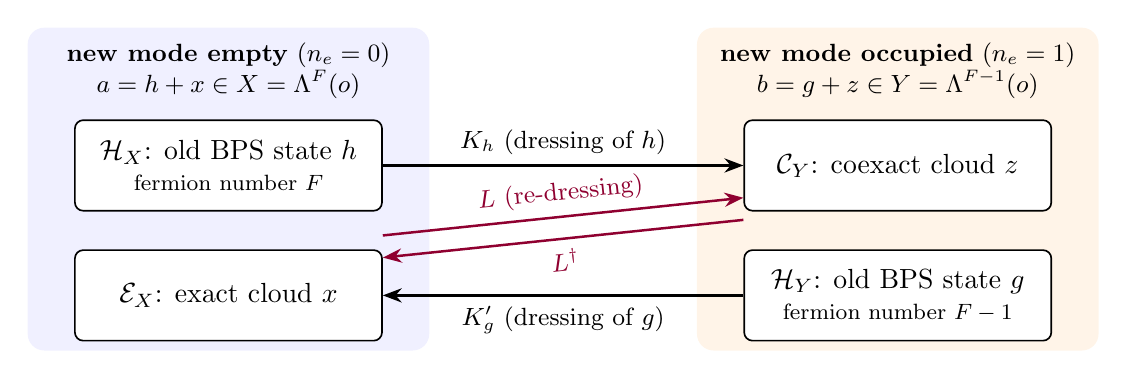
\begin{tikzpicture}[
  box/.style={draw, rounded corners=3pt, minimum width=3.9cm, minimum height=1.15cm, align=center, line width=0.6pt, fill=white},
  >={Stealth[length=2.4mm]}]
\fill[blue!6, rounded corners=6pt] (-2.55,-1.05) rectangle (2.55,3.05);
\fill[orange!9, rounded corners=6pt] (5.95,-1.05) rectangle (11.05,3.05);
\node[font=\small, align=center] at (0,2.5) {\textbf{new mode empty} ($n_e=0$)\\ $a=h+x\in X=\Lambda^F(o)$};
\node[font=\small, align=center] at (8.5,2.5) {\textbf{new mode occupied} ($n_e=1$)\\ $b=g+z\in Y=\Lambda^{F-1}(o)$};
\node[box] (HX) at (0,1.3) {$\Hc_X$: old BPS state $h$\\[-1pt]\footnotesize fermion number $F$};
\node[box] (EX) at (0,-0.35) {$\Ec_X$: exact cloud $x$};
\node[box] (CY) at (8.5,1.3) {$\Cc_Y$: coexact cloud $z$};
\node[box] (HY) at (8.5,-0.35) {$\Hc_Y$: old BPS state $g$\\[-1pt]\footnotesize fermion number $F-1$};
\draw[->, line width=0.9pt] (HX.east) -- node[above, font=\small] {$K_h$ (dressing of $h$)} (CY.west);
\draw[->, line width=0.9pt] (HY.west) -- node[below, font=\small] {$K'_g$ (dressing of $g$)} (EX.east);
\draw[->, line width=0.9pt, purple!75!black] ([yshift=5pt]EX.north east) -- node[above, sloped, font=\small] {$L$ (re-dressing)} ([yshift=5pt]CY.south west);
\draw[->, line width=0.9pt, purple!75!black] ([yshift=-3pt]CY.south west) -- node[below, sloped, font=\small] {$L^\dagger$} ([yshift=-3pt]EX.north east);
\end{tikzpicture}
\caption{Structure of the exact uplift (\S\S\ref{sec:uplift}--\ref{sec:antiherm}). A BPS state of the enlarged model
is assembled from old BPS states $h$ and $g$ plus two dressing clouds. The decoder eigenvalue is the fraction of the norm
in the left column. An old state $h$ is dressed into the occupied sector by $K_h$, which lowers its decoder eigenvalue
from $1$ to $1/(1+\sigma^2)$ at first order. The coupling $L$ returns part of the cloud to the empty sector as an exact
form, raising the eigenvalue again; by the adjoint relation the return map is $L^\dagger$. The $g$-states are the mirror
image. The two families communicate only through $L$.}
\label{fig:schematic}
\end{figure}

\subsection{Orthogonal splitting}

Define the two families of uplifted states,
\begin{equation}\label{eq:families}
B_h=\{\Psi(h,0):h\in\Hc_X\},\qquad B_g=\{\Psi(0,g):g\in\Hc_Y\}.
\end{equation}
Equivalently, $B_h$ consists of the BPS states whose occupied-sector component $b$ has no harmonic part, and $B_g$ of
those whose empty-sector component $a$ has no harmonic part. By Theorem~\ref{thm:uplift}, $B=B_h+B_g$. The two families
are in fact orthogonal.

\begin{theorem}[Orthogonal splitting]\label{thm:split}\VER\
$B=B_h\oplus B_g$ with $B_h\perp B_g$.
\end{theorem}

\begin{proof}
Let $\Psi_h=\Psi(h,0)$, with clouds $(x_h,z_h)$, and $\Psi_g=\Psi(0,g)$, with clouds $(x_g,z_g)$. The harmonic parts are
orthogonal to everything else, so
$\ip{\Psi_h}{\Psi_g}=\ip{h+x_h}{x_g}+\ip{z_h}{g+z_g}=\ip{x_h}{x_g}+\ip{z_h}{z_g}$. This is the inner product of the
cloud vectors, $\big((1+\LL)^{-1}s_h,(1+\LL)^{-1}s_g\big)$, with sources $s_h=(0,-\eps\Kh h)$ and $s_g=(\eps\Kg g,0)$.
Using $\LL^\dagger=-\LL$,
\[
\ip{(1+\LL)^{-1}s_h}{(1+\LL)^{-1}s_g}=\ip{s_h}{\big[(1+\LL)(1-\LL)\big]^{-1}s_g}=\ip{s_h}{\mathrm{diag}\big((1+R')^{-1},(1+R)^{-1}\big)\,s_g}=0,
\]
because the middle operator is block-diagonal while $s_h$ and $s_g$ live in different blocks.
\end{proof}

\noindent The orthogonality can also be seen directly from the BPS equations~\eqref{eq:bps}, without solving them. Write
$b_h=Q_0^\dagger v$ (it is coexact) and $a_g=Q_0w$ (it is exact). Then
$\ip{a_h}{a_g}=\ip{Q_0^\dagger a_h}{w}=\eps\ip{E^\dagger b_h}{w}=\eps\ip{b_h}{Ew}$, while
$\ip{b_h}{b_g}=\ip{v}{Q_0b_g}=-\eps\ip{v}{Ea_g}=-\eps\ip{v}{Q_0Ew}=-\eps\ip{b_h}{Ew}$. The two contributions cancel. The
numerical overlap between the two families is $\le1.1\times10^{-15}$ at $\Np=9$--$15$.

The splitting also fixes the uplift of an old state uniquely. In CV's cohomological language, a BPS state of the enlarged
model uplifts the old class $[h]$ if its empty-sector component $a$ is in the class $[h]$, i.e.\ if the harmonic part of
$a$ is $h$. By Theorem~\ref{thm:uplift} these states are exactly $\Psi(h,g)$ for arbitrary $g\in\Hc_Y$. The freedom in
$g$ is CV's coset ambiguity (their eq.~(40)), and the need to pick harmonic representatives is their second ambiguity.

\begin{corollary}[Canonical uplift]\label{cor:minnorm}\DER\
Among all BPS states of the enlarged model that uplift the old BPS state $h$, the state $\Psi(h,0)$ is the unique one of
minimum norm. Equivalently, it is the unique one orthogonal to every BPS state uplifted from the occupied sector.
\end{corollary}

\begin{proof}
$\Psi(h,g)=\Psi(h,0)+\Psi(0,g)$ by linearity, and $\Psi(h,0)\perp\Psi(0,g)$ by Theorem~\ref{thm:split}. Hence
$\|\Psi(h,g)\|^2=\|\Psi(h,0)\|^2+\|\Psi(0,g)\|^2$, which is minimal exactly when $\Psi(0,g)=0$, i.e.\ $g=0$.
\end{proof}

\begin{remark}
The one-sided half of the construction, solving only $b=g-\eps Ka$ for closedness, has the form of the classical
homological perturbation lemma for $Q=Q_0+(\eps E)(\cdot\wedge e)$, with the Hodge homotopy $Q_0^+$. The BPS condition
adds the dual half. We have not yet checked whether the two-sided, anti-Hermitian form or the orthogonal splitting
appears in the literature.
\end{remark}

%=====================================================================
\section{The decoder in closed form}\label{sec:decoder}
%=====================================================================

\subsection{Norms and decoder forms}

By~\eqref{eq:decoder-forms}, the decoder is determined by two quadratic forms on $B$, the norm $\|\Psi\|^2$ and the
reflection form $\ip{\Psi}{U\Psi}=\|a\|^2-\|b\|^2$. With $a=h+x$ and $b=g+z$ and the orthogonality of the Hodge pieces,
\begin{equation}\label{eq:forms}
\|\Psi\|^2=\|h\|^2+\|x\|^2+\|g\|^2+\|z\|^2,\qquad
\ip{\Psi}{U\Psi}=\|h\|^2+\|x\|^2-\|g\|^2-\|z\|^2 .
\end{equation}
We evaluate them on the two families using~\eqref{eq:xz}.

\paragraph{The $h$-family.} Put $k=\Kh h\in\Cc_Y$, the first-order cloud of $h$. With $g=0$,
$z_h=-\eps(1+R)^{-1}k$, and by the push-through identity $(1+L^\dagger L)^{-1}L^\dagger=L^\dagger(1+LL^\dagger)^{-1}$,
$x_h=-L^\dagger(1+R)^{-1}k$. Hence
\begin{equation}\label{eq:hfam}
\|z_h\|^2=\ip{k}{(1+R)^{-2}k},\qquad \|x_h\|^2=\ip{k}{R(1+R)^{-2}k},
\end{equation}
so that
\begin{equation}\label{eq:hfam2}
\|\Psi_h\|^2=\|h\|^2+\ip{k}{(1+R)^{-1}k},\qquad \ip{\Psi_h}{U\Psi_h}=\|h\|^2-\ip{k}{(1-R)(1+R)^{-2}k}.
\end{equation}
Read in the eigenbasis of $R$, these formulas say what re-dressing does. A component of the first-order cloud along an
eigenvector of $R$ with eigenvalue $\rho$ has its norm reduced from $1$ to $1/(1+\rho)$. Of that, a fraction $1/(1+\rho)$
stays in the occupied sector and a fraction $\rho/(1+\rho)$ returns to the empty sector.

\paragraph{The $g$-family.} Put $k'=\Kg g\in\Ec_X$. Then $x_g=\eps(1+R')^{-1}k'$ and $z_g=-L(1+R')^{-1}k'$, and in the
same way
\begin{equation}\label{eq:gfam}
\|\Psi_g\|^2=\|g\|^2+\ip{k'}{(1+R')^{-1}k'},\qquad \ip{\Psi_g}{U\Psi_g}=-\|g\|^2+\ip{k'}{(1-R')(1+R')^{-2}k'}.
\end{equation}

\paragraph{The cross term.} Since $\Psi_h\perp\Psi_g$ (Theorem~\ref{thm:split}), $\ip{b_h}{b_g}=-\ip{a_h}{a_g}$ and
therefore
\begin{equation}\label{eq:cross}
\ip{\Psi_h}{U\Psi_g}=2\ip{a_h}{a_g}=2\ip{x_h}{x_g}=-2\eps\,\ip{k}{L(1+R')^{-2}k'} .
\end{equation}
The two families are orthogonal, but the decoder couples them through the re-dressing map $L$.

\subsection{The block pencil}

Choose orthonormal bases $\{h_i\}$ of $\Hc_X$ and $\{g_j\}$ of $\Hc_Y$, and parametrize $B$ by the coefficient vector
$v$ of $\Psi=\sum_iv_i\Psi(h_i,0)+\sum_jv_{b_F+j}\Psi(0,g_j)$. The Rayleigh quotient of the reflection is
$\ip{\Psi}{U\Psi}/\|\Psi\|^2=v^\dagger\mathcal Nv/v^\dagger\mathcal Gv$, with matrices read off from
\eqref{eq:hfam2}--\eqref{eq:cross}.

\begin{proposition}[Closed-form decoder]\label{prop:pencil}\VER\
The decoder eigenvalues are $\lambda=(1+\mu)/2$, where $\mu$ runs over the generalized eigenvalues of the pencil
$\mathcal Nv=\mu\,\mathcal Gv$ on $\Hc_X\oplus\Hc_Y$. The Gram matrix is block-diagonal,
\begin{equation}\label{eq:pencilG}
\mathcal G=\begin{pmatrix}\mathcal G_{hh}&0\\0&\mathcal G_{gg}\end{pmatrix},\qquad
\mathcal G_{hh}=1+\Kh^\dagger(1+R)^{-1}\Kh,\qquad \mathcal G_{gg}=1+\Kg^\dagger(1+R')^{-1}\Kg ,
\end{equation}
while the reflection matrix $\mathcal N=\big(\begin{smallmatrix}\mathcal N_{hh}&\mathcal N_{hg}\\ \mathcal N_{hg}^\dagger&\mathcal N_{gg}\end{smallmatrix}\big)$ has blocks
\begin{equation}\label{eq:pencil}
\mathcal N_{hh}=1-\Kh^\dagger\,\frac{1-R}{(1+R)^2}\,\Kh,\qquad
\mathcal N_{gg}=-1+\Kg^\dagger\,\frac{1-R'}{(1+R')^2}\,\Kg,\qquad
\mathcal N_{hg}=-2\eps\,\Kh^\dagger L\,(1+R')^{-2}\,\Kg .
\end{equation}
\end{proposition}

The pencil reproduces the eigenvalues of the exact $\Np$-mode decoder to $10^{-10}$
(\path{tests/test_uplift.py}). All its ingredients, $\Kh$, $\Kg$ and $L$, are maps of the \emph{old} model.

\subsection{First order: the principal angle is the arctangent of the dressing amplitude}

If the re-dressing map is neglected, $L\to0$, the clouds reduce to their sources, $x=\eps\Kg g$ and $z=-\eps\Kh h$. This is
the solution of~\eqref{eq:uplift} to first order in the new couplings $\eta$. Both $\mathcal G$ and $\mathcal N$ become
block-diagonal, with $\mathcal G=1+\Kh^\dagger\Kh$ and $\mathcal N=1-\Kh^\dagger\Kh$ on the $h$-block. In the basis of
right singular vectors of $\Kh$, with singular values $\sigma_j$, both are diagonal and $\mu_j=(1-\sigma_j^2)/(1+\sigma_j^2)$.
The $g$-block works the same way with $\sigma'_j$ and an overall sign.

\begin{corollary}[First-order decoder]\label{cor:first}\VER\
To first order in the new couplings, the decoder eigenvalues are
\begin{equation}\label{eq:first}
\lambda^{(1)}_{h,j}=\frac{1}{1+\sigma_j^2}=\cos^2\theta_j,\quad \tan\theta_j=\sigma_j;\qquad\qquad
\lambda^{(1)}_{g,j}=\frac{\sigma_j'^2}{1+\sigma_j'^2},\quad \theta_j=\tfrac\pi2-\arctan\sigma'_j .
\end{equation}
\end{corollary}

This is the simplest result of the report, and the one used most below. To first order, \emph{the principal angle between an
uplifted old BPS state and the empty sector is the arctangent of its dressing amplitude}. A state that needs no
dressing ($\sigma=0$) sits on the wall $\lambda=1$. A state whose dressing has unit norm ($\sigma=1$) sits at
$\lambda=\tfrac12$. The quantity $\tan^2\theta=1/\lambda-1$ is CV's dressing cost $\kappa=m_{-1}-1$ (their eq.~(61)). So
$\sigma_j^2$ is CV's dressing cost of the singular vector $h_j$, evaluated at first order. The decoder spectrum at first order
is a direct image of the distribution of dressing costs over old BPS states.

The singular values are not small: $\eta$ has the same coupling variance as $\omega_0$, and in the bulk of the spectrum
$\sigma=O(1)$. ``First order'' therefore does not mean ``small angle''. It means that each old state is dressed once, while
its cloud is not re-dressed.

\subsection{Re-dressing is monotone}

\begin{proposition}[Monotone self-dressing]\label{prop:monotone}\VER\
Keep the diagonal blocks of the pencil~\eqref{eq:pencilG}--\eqref{eq:pencil} and drop the off-diagonal block. Then every ordered eigenvalue of the
$h$-block lies at or above its first-order value $1/(1+\sigma_j^2)$, and every ordered eigenvalue of the $g$-block lies
at or below $\sigma_j'^2/(1+\sigma_j'^2)$.
\end{proposition}

\begin{proof}
On the $h$-block, the quantity $1-\lambda=\|b\|^2/\|\Psi\|^2$ has Rayleigh quotient, by~\eqref{eq:hfam}--\eqref{eq:hfam2},
\[
1-\lambda(h)=\frac{n}{\|h\|^2+m},\qquad n=\ip{k}{(1+R)^{-2}k},\quad m=\ip{k}{(1+R)^{-1}k},\quad k=\Kh h .
\]
Since $R\ge0$ we have $n\le m\le\|k\|^2$. Because $t\mapsto t/(c+t)$ is increasing, $n/(c+m)\le m/(c+m)\le\|k\|^2/(c+\|k\|^2)$ with
$c=\|h\|^2$. The right-hand side is the first-order quotient. The inequality between the two Rayleigh quotients holds
for every $h$. By the Courant--Fischer min-max principle for generalized eigenproblems, it carries over to the ordered
eigenvalues. The $g$-block is identical, with the roles of the sectors exchanged.
\end{proof}

Re-dressing therefore pushes the $h$-states towards $\lambda=1$ and the $g$-states towards $\lambda=0$. It makes the decoder
more decisive than first order. The off-diagonal block has a definite effect too. In orthonormal bases of $B_h$ and $B_g$,
$PUP=\big(\begin{smallmatrix}M_h&C\\ C^\dagger&M_g\end{smallmatrix}\big)$, and
\begin{equation}\label{eq:T2mix}
T_2=\frac1d\Big[\tr M_h^2+\tr M_g^2+2\,\|C\|_F^2\Big]\;\ge\;\frac1d\Big[\tr M_h^2+\tr M_g^2\Big],
\end{equation}
so the coupling between the families can only increase $T_2$. Both effects raise $T_2$ above its first-order value
(\S\ref{sec:why}).

\paragraph{A symmetry at even $\Np$ \NUM.} For even $\Np$ the old model has an odd number of modes, and
$b_F=b_{F-1}$. Numerically, the spectrum of $M_g$ is exactly minus that of $M_h$ in each realization, to $7\times10^{-15}$
at $\Np=10,12,14$. So the familiar $\lambda\leftrightarrow1-\lambda$ symmetry of the even-$\Np$ decoder acts block by
block, exchanging the two families. For odd $\Np$ there is no such symmetry: all $g$-states sit on the occupied side,
$\mu_g\le-0.21$.

%=====================================================================
\section{The dressing cost is a time-integrated two-point function}\label{sec:twopoint}
%=====================================================================

The first-order decoder is fixed by the singular values of $\Kh$ and $\Kg$. These have a direct physical meaning.

\begin{proposition}[Dressing cost]\label{prop:twopoint}\VER\
The squared singular values $\sigma_j^2$ are the eigenvalues of the operator on the old BPS space $\Hc_X$
\begin{equation}\label{eq:Dh}
\mathcal D_h=P_{\Hc}\,E^\dagger H_0^{-1}E\,P_{\Hc}=\int_0^\infty d\tau\;P_{\Hc}\,E^\dagger e^{-\tau H_0}E\,P_{\Hc},
\end{equation}
where $H_0$ is the old Hamiltonian. Likewise $\sigma_j'^2$ are the eigenvalues of
$P_{\Hc}\,E\,H_0^{-1}E^\dagger P_{\Hc}$ on $\Hc_Y$.
\end{proposition}

\begin{proof}
$\Kh^\dagger\Kh=P_{\Hc}E^\dagger(Q_0^+)^\dagger Q_0^+EP_{\Hc}=P_{\Hc}E^\dagger(Q_0Q_0^\dagger)^+EP_{\Hc}$. For $h\in\Hc_X$ the
form $Eh$ is exact, as shown in \S\ref{sec:uplift}. On exact forms $Q_0$ vanishes, so $H_0=Q_0Q_0^\dagger$ there. In
degree $F+2$, $H_0$ has no zero modes because there is no cohomology, so it is invertible on $\Ec^{F+2}$ and
$(Q_0Q_0^\dagger)^+Eh=H_0^{-1}Eh$. The integral representation is $H_0^{-1}=\int_0^\infty e^{-\tau H_0}d\tau$ on this
gapped subspace. The statement for $\Kg$ is the same with coexact forms in degree $F-3$, where $H_0=Q_0^\dagger Q_0$.
\end{proof}

For a normalized old BPS state $h$, the diagonal element is
\begin{equation}\label{eq:twopoint}
\ip{h}{\mathcal D_h h}=\int_0^\infty d\tau\,\big\langle h\big|E^\dagger(\tau)E(0)\big|h\big\rangle
=\sum_{n}\frac{|\langle n|E|h\rangle|^2}{\nu_n},\qquad E(\tau)=e^{\tau H_0}Ee^{-\tau H_0},
\end{equation}
using $H_0h=0$. Here the sum runs over the eigenstates $|n\rangle$ of the old model at fermion number $F+2$, with
energies $\nu_n>0$. This is a zero-temperature Euclidean two-point function of the operator $E$ in the BPS state $h$,
integrated over the Euclidean time separation. Equivalently, it is the second-order energy-denominator sum for the state
$E h$, which has no zero-energy component.

The operator $E=\sum_{i<j}C_{ije}c_i^\dagger c_j^\dagger$ has Gaussian couplings that are independent of the old
Hamiltonian's. In double-scaled language it is a random \emph{matter} operator made of two fermions, with R-charge $2/\hat q$ since
each fermion carries $1/\hat q$~\cite{FGMS}. Proposition~\ref{prop:twopoint} therefore says the following. \emph{The decoder spectrum
at first order is the spectrum, as an operator on the old BPS space and not just its trace, of the time-integrated
zero-temperature two-point function of a matter operator.} Our previous calculations of $T_2$ were
of the same type, but without the time integral and with $n_e$ in place of $E$. They involved the BPS-to-BPS two-point
function of $n_e$ evaluated by LMRS and BLY methods~\cite{LMRS,BLY,prog0929}. Here the matter operator maps the BPS sector into
a charge sector without BPS states. The integral therefore converges, with the gap of that sector as its infrared
cutoff.

How much of the exact decoder is controlled by such two-point functions? Let
$\mathcal D=E^\dagger H_0^{-1}E$ on the closed forms of degree $F$, and $\mathcal D'=EH_0^{-1}E^\dagger$ on the coclosed
forms of degree $F-1$. Then $\Kh^\dagger\Kh$, $\Kh^\dagger L$ and $R'$ are the blocks of $\mathcal D$ on
$\Hc_X\oplus\Ec_X$, and $\Kg^\dagger\Kg$ and $R$ are blocks of $\mathcal D'$. By push-through,
$A^\dagger f(ABA^\dagger)A=A^\dagger A\,f(BA^\dagger A)$. For example $\Kh^\dagger(1+R)^{-1}\Kh=[\mathcal D(1+P_{\Ec}\mathcal D)^{-1}]_{\Hc\Hc}$
(checked to $3\times10^{-15}$). So both diagonal blocks of the pencil~\eqref{eq:pencilG}--\eqref{eq:pencil} are functionals of the integrated
two-point functions $\mathcal D$ and $\mathcal D'$ alone. The off-diagonal block also needs the map $\Kg$ itself, which
links the two sides.

%=====================================================================
\section{The walls}\label{sec:walls}
%=====================================================================

\subsection{Exact walls are kernels of the pair operator}

\begin{proposition}[Exact walls]\label{prop:walls}\VER\
An eigenvector of the decoder has $\lambda=1$ if and only if it is $\Psi=h$ with $h\in\Hc_X$ and $Eh=0$. It has $\lambda=0$
if and only if it is $\Psi=g\wedge e$ with $g\in\Hc_Y$ and $E^\dagger g=0$.
\end{proposition}

\begin{proof}
$\lambda=1$ means $b=0$, i.e.\ $g=0$ and $z=0$. With $g=0$, \eqref{eq:xz} gives $z=-\eps(1+R)^{-1}\Kh h$, which vanishes
iff $\Kh h=Q_0^+Eh=0$. Since $Eh$ is exact and $Q_0^+$ is injective on exact forms, this holds iff $Eh=0$. Then $x=0$ as
well, so $\Psi=h$. The case $\lambda=0$ is symmetric.
\end{proof}

At the walls the uplift is therefore \emph{bare}: the old BPS state is a BPS state of the enlarged model as it stands.
In CV's terms these are the old states whose bare embedding is already BPS, so that their dressing cost vanishes. They
require $h$ to lie in the kernel of $E=\eta\wedge$, a structure of Lefschetz type. By the hard Lefschetz property of a
generic 2-form, $E:\Lambda^F(o)\to\Lambda^{F+2}(o)$ is surjective in our degree, and its kernel fills a large part of
$\Lambda^F(o)$: 64\,\%, 46\,\% and 58\,\% at $\Np=12$, $13$ and $14$. The question is how much of the small subspace $\Hc_X$ it
captures.

Near the walls, first-order theory is accurate. At $\Np=14$ the upper quantiles ($q\ge0.75$) of the exact decoder agree with $1/(1+\sigma^2)$ to
$\le3\times10^{-3}$. Eigenvectors with $\lambda\ge0.97$ have 99\,\% of their norm in $\Hc_X$, and their ratio
$\|Eh\|/\|h\|$ is about $1.1$, against 4--8 in the bulk.

\subsection{Counting the atoms}

How many exact wall states are there? Since $Eh$ is exact, $E$ maps $\Hc_X$ into $\Ec^{F+2}$. The latter has dimension
$e_{F+2}$, which the exactness of the old complex above the BPS window fixes recursively,
\begin{equation}\label{eq:ek}
e_k=\binom Nk-e_{k+3}\qquad(e_k=0\ \text{for } k>N),
\end{equation}
because $\Lambda^k=\Ec^k\oplus\Cc^k$ and $Q_0$ maps $\Cc^k$ bijectively onto $\Ec^{k+3}$. The rank of $E$ on $\Hc_X$
is at most $e_{F+2}$, so its kernel has dimension at least $b_F-e_{F+2}$. With the analogous bound for the occupied wall,
using coexact forms of degree $F-3$, we obtain a lower bound on the number of exact atoms. Table~\ref{tab:dims} compares it
with the measured counts. The bound is saturated for $\Np\le10$. Beyond that there is a small, deterministic excess:
$+1$, $+2$, $+14$, $+28$ at $\Np=11$--$14$, identical in every realization. We do not yet understand this excess. It
implies further algebraic constraints on how $\Hc_X$ sits relative to $\ker E$.

\begin{table}[ht]
\centering\small
\caption{Dimensions, the hard-edge ratio $r=e_{F+2}/b_F$, and exact atom counts (both walls) against the lower bound.}
\label{tab:dims}
\begin{tabular}{lrrrrrrrrr}\toprule
$\Np$ & 8 & 9 & 10 & 11 & 12 & 13 & 14 & 15 & 16\\\midrule
$D$ & 70 & 126 & 252 & 462 & 924 & 1716 & 3432 & 6435 & 12870\\
$d$ & 54 & 81 & 162 & 243 & 486 & 729 & 1458 & 2187 & 4374\\
$b_F$ & 27 & 54 & 81 & 162 & 243 & 486 & 729 & 1458 & 2187\\
$b_{F-1}$ & 27 & 27 & 81 & 81 & 243 & 243 & 729 & 729 & 2187\\
$e_{F+2}$ & 7 & 28 & 36 & 119 & 164 & 483 & 702 & 1911 & 2898\\
$r=e_{F+2}/b_F$ & 0.26 & 0.52 & 0.44 & 0.74 & 0.68 & 0.99 & 0.96 & 1.31 & 1.33\\
atoms (measured) & 40 & 45 & 90 & 80 & 160 & 41 & 82 & 0 & 0\\
atoms (bound) & 40 & 45 & 90 & 79 & 158 & 27 & 54 & 0 & 0\\\bottomrule
\end{tabular}
\end{table}

\subsection{The hard edge and its collapse}\label{sec:hardedge}

The same count controls the states \emph{near} the walls. When $r=e_{F+2}/b_F<1$, the map $E|_{\Hc_X}$ has a forced
kernel: exact atoms. When $r$ is close to $1$, the map is nearly square. As for a square random matrix, its smallest
singular values then pile up near zero, giving many dressing costs close to $0$ and a hard edge of decoder eigenvalues at
the wall. When $r$ is well above $1$, the map is ``tall'' and its smallest singular value is bounded away from zero. The
hard edge then disappears \INTERP. The ratio is $0.99$ and $0.96$ at $\Np=13,14$ but jumps to $1.31$ at $\Np=15$
(Table~\ref{tab:dims}). Since $b_F\sim3^{N/2}$ while $e_{F+2}$ grows like $2^N/\sqrt N$, $r$ keeps growing, and near-wall
states should be absent for all larger $\Np$.

\PRE\ Before computing the $\Np=15$ decoder, we used the first-order formula~\eqref{eq:first}, computed from the
$N=14$ model alone, to predict the fraction of eigenvalues within $10^{-3}$ of a wall. It predicted a drop from $0.117$
at $\Np=14$ to $0.003$--$0.012$ at $\Np=15$. The exact values are $0.128$ and $0.012$--$0.023$ (six realizations).
Figure~\ref{fig:walls}(a) shows the collapse, together with first order and the exact atoms. First order runs about
10\,\% low at $\Np=13$--$14$ and about a factor of 2 low after the collapse, where only a few near-wall states remain. The walls are an arithmetic phenomenon, and they are essentially gone from $\Np=15$ on.

\begin{figure}[t]
\centering
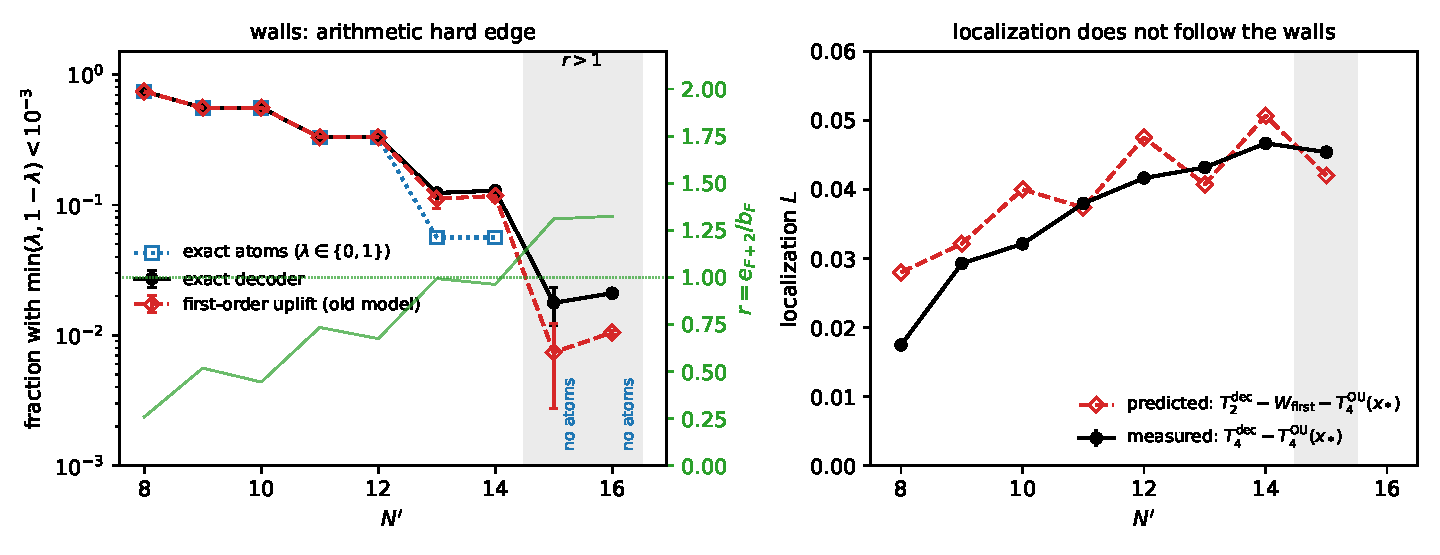
\includegraphics[width=\textwidth]{progress_2026-10-13_figs/fig_walls_vs_localization.pdf}
\caption{(a)~Fraction of decoder eigenvalues within $10^{-3}$ of a wall: exact (black, range over realizations),
first-order prediction from the old model (red), and exact atoms (blue). Green, right axis: the dimension ratio
$r=e_{F+2}/b_F$, which crosses $1$ between $\Np=14$ and $15$ (shaded). (b)~Localization $L=T_4^\dec-T_4^\OU(x_*)$ measured
(black) and predicted from the first-order heterogeneity (red; \S\ref{sec:prediction}). It does not drop when the walls
collapse at $\Np=15$ (shaded).}
\label{fig:walls}
\end{figure}

%=====================================================================
\section{The fourth moment is a heterogeneity}\label{sec:fourth}
%=====================================================================

\subsection{An identity}\label{sec:identity}

The variable $y=\cos^22\theta$ lies in $[0,1]$, so $y^2=y-y(1-y)$. Averaging,
\begin{equation}\label{eq:identity}
T_4=T_2-W,\qquad W\equiv\langle y(1-y)\rangle=\tfrac14\langle\sin^24\theta\rangle .
\end{equation}
The function $y(1-y)=\tfrac14\sin^24\theta$ vanishes at $\theta=0$, $\pi/4$ and $\pi/2$, i.e.\ at $\lambda=1$, $\tfrac12$
and $0$. It is maximal at $\theta=\pi/8$ and $3\pi/8$, i.e.\ at $\lambda=\cos^2(\pi/8)\approx0.854$ and $0.146$. $W$ is
therefore the weight of the decoder spectrum at \emph{intermediate} angles, away from both walls and from the balanced
point $\lambda=\tfrac12$. We call it the heterogeneity. At fixed $T_2$, a larger fourth moment means a smaller $W$.

Applied to the definition~\eqref{eq:L} of localization, at equal $T_2$,
\begin{equation}\label{eq:LW}
L=T_4^\dec-T_4^\OU(x_*)=W^\OU(x_*)-W^\dec .
\end{equation}
\emph{Localization is exactly the decoder's deficit of intermediate angles relative to an isotropic deformation with the
same second moment.} This can be seen directly in the angle distributions. Figure~\ref{fig:densities} compares the
distribution of $y$ for the decoder with that of the isotropic pair $(P,P_x)$ at the lag closest to $x_*$. The decoder has
more weight at both ends ($y\approx0$ and $y\approx1$) and less in between.

\begin{figure}[t]
\centering
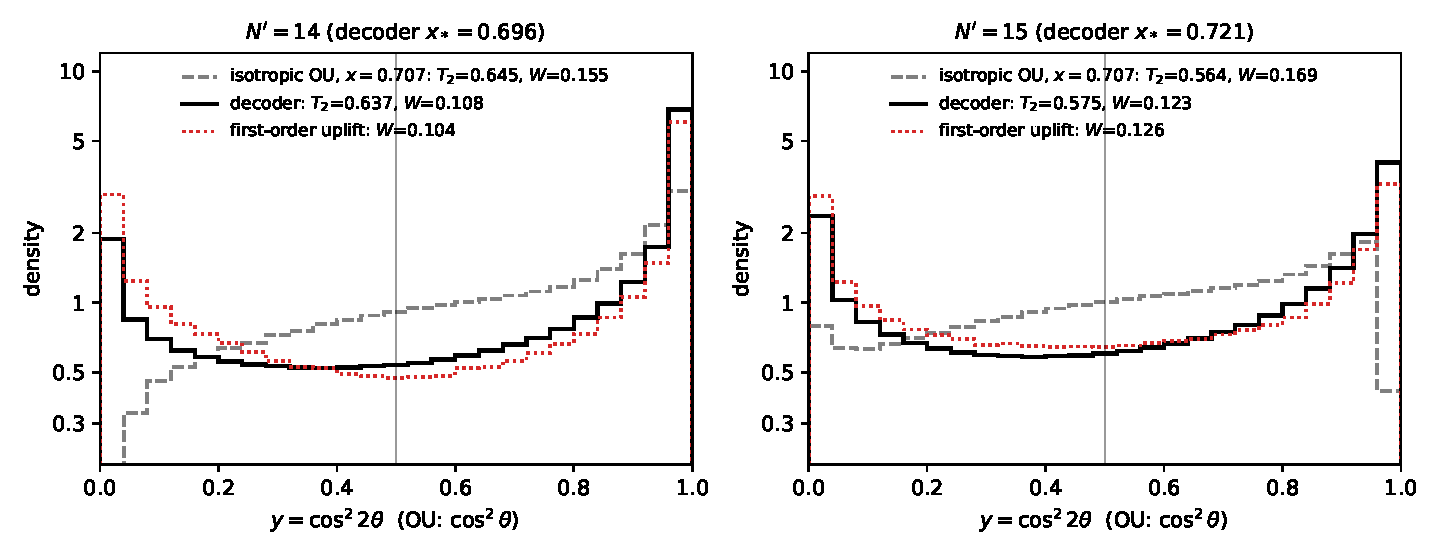
\includegraphics[width=\textwidth]{progress_2026-10-13_figs/fig_angle_densities.pdf}
\caption{What localization is. Distribution of $y$ for the decoder (black) and of the corresponding variable
$\cos^2\theta$ for the isotropic OU pair $(P,P_x)$ (gray). The OU lag is the stored one closest to the matched $x_*$; its
$T_2$ differs from the decoder's by about $0.01$, as quoted in the legends. Red: the first-order prediction from the old
model, $y=((1-\sigma^2)/(1+\sigma^2))^2$. The decoder is depleted at intermediate angles and enhanced at both ends, and the
first-order prediction reproduces this shape. $W$ is the heterogeneity of~\eqref{eq:identity}.}
\label{fig:densities}
\end{figure}

\subsection{The walls are not the explanation}\label{sec:walls-refuted}

Equation~\eqref{eq:LW} leaves open \emph{which} part of the spectrum produces the deficit. In the previous report, and
after finding the hard edge (\S\ref{sec:hardedge}), our working hypothesis was the walls. States pressed against
$\lambda\in\{0,1\}$ have $y\approx1$, where $y(1-y)$ is small, and an isotropic deformation does not produce such a pile-up.
This hypothesis makes a sharp prediction: since the walls collapse at $\Np=15$, localization should drop there.

\PRE\ We recorded this prediction and then extended the OU campaign of~\cite{prog1005} to $\Np=15$. There were 8
samples, two memory-capped jobs, and $K=8$ lags. The lag-interpolation error of $K=8$ was checked at $\Np=12$--$14$ to be
$\le2\times10^{-4}$. The result is $T_2^\dec=0.5754$, $T_4^\dec=0.4524$, $x_*=0.721$ and $T_4^\OU(x_*)=0.4070$, so
\[
L(\Np=15)=0.0454\pm0.0003,
\]
compared with $0.0432$ and $0.0467$ at $\Np=13$ and $14$ (Figure~\ref{fig:walls}b). The prediction is refuted.
Localization is a property of the bulk of the angle distribution, not of the walls. Its share of $T_4^\dec-T_4^{\rm free}$ is
17\,\%, against 77\,\% for free liberation and 5.8\,\% for the isotropic non-freeness.

\subsection{Predicting the heterogeneity from the old model}\label{sec:prediction}

If localization lives in the bulk, the natural first guess is the first-order decoder of
Corollary~\ref{cor:first}. Substituting \eqref{eq:first} into $y(1-y)$ gives, with $s=\sigma^2$,
\[
y=\Big(\frac{1-s}{1+s}\Big)^2,\qquad 1-y=\frac{4s}{(1+s)^2},\qquad
y(1-y)=w(s)\equiv\frac{4s(1-s)^2}{(1+s)^4},
\]
and the same function of $s=\sigma'^2$ for the $g$-states. The first-order heterogeneity is thus a single average over
the dressing costs of the old model,
\begin{equation}\label{eq:W1}
\Wone=\frac1d\Big[\sum_{j=1}^{b_F}w(\sigma_j^2)+\sum_{j=1}^{b_{F-1}}w(\sigma_j'^2)\Big].
\end{equation}
The weight $w(s)=\tfrac14\sin^2(4\arctan\sqrt s)$ vanishes for protected states ($s=0$), for balanced states ($s=1$) and
for heavily dressed states ($s\to\infty$). It is maximal at $s=\tan^2(\pi/8)\approx0.17$ and $s=\tan^2(3\pi/8)\approx5.8$.

We therefore predict
\begin{equation}\label{eq:prediction}
T_4^\dec\;\approx\;T_2^\dec-\Wone,\qquad
L\;\approx\;L^{(1)}\equiv T_2^\dec-\Wone-T_4^\OU(x_*).
\end{equation}
Here $\Wone$ comes from the $N=\Np-1$ model only (13 realizations for $\Np\le14$, 6 at $\Np=15$). $T_2^\dec$ and
$T_4^\OU(x_*)$ are measured in the OU campaign of~\cite{prog1005}, extended here to $\Np=15$. Table~\ref{tab:prediction} and
Figure~\ref{fig:heterogeneity} show the result.

\begin{table}[ht]
\centering\small
\caption{Prediction of the decoder's fourth moment from the first-order dressing costs of the old model,
eq.~\eqref{eq:prediction}. ``Error'' is predicted minus measured. For comparison, the errors of free liberation and of
the isotropic OU curve at the decoder's $T_2$ are also given; the OU error equals $-L$ by definition. All values are
all-site averages.}
\label{tab:prediction}
\setlength{\tabcolsep}{4.5pt}
\begin{tabular}{lcccccccc}\toprule
$\Np$ & $W^\dec$ & $\Wone$ & $T_4^\dec$ & $T_2^\dec-\Wone$ & error & lib.\ error & OU error & $L$ / $L^{(1)}$\\\midrule
8  & 0.0396 & 0.0291 & 0.7778 & 0.7884 & $+0.0105$ & $-0.0151$ & $-0.0175$ & 0.0175 / 0.0280\\
9  & 0.0653 & 0.0625 & 0.6666 & 0.6694 & $+0.0029$ & $-0.0312$ & $-0.0293$ & 0.0293 / 0.0322\\
10 & 0.0666 & 0.0587 & 0.6790 & 0.6869 & $+0.0079$ & $-0.0315$ & $-0.0321$ & 0.0321 / 0.0400\\
11 & 0.0891 & 0.0897 & 0.5799 & 0.5793 & $-0.0006$ & $-0.0444$ & $-0.0380$ & 0.0380 / 0.0374\\
12 & 0.0897 & 0.0838 & 0.5964 & 0.6023 & $+0.0059$ & $-0.0446$ & $-0.0417$ & 0.0417 / 0.0475\\
13 & 0.1083 & 0.1107 & 0.5101 & 0.5077 & $-0.0025$ & $-0.0539$ & $-0.0432$ & 0.0432 / 0.0408\\
14 & 0.1085 & 0.1045 & 0.5283 & 0.5323 & $+0.0040$ & $-0.0541$ & $-0.0467$ & 0.0467 / 0.0507\\
15 & 0.1230 & 0.1264 & 0.4524 & 0.4490 & $-0.0034$ & $-0.0606$ & $-0.0454$ & 0.0454 / 0.0420\\\bottomrule
\end{tabular}
\end{table}

\NUM\ For $\Np\ge9$ the prediction misses $T_4$ by at most $0.008$, and by at most $0.006$ for $\Np\ge11$. Free liberation
misses by $0.03$--$0.06$, and the isotropic curve misses by the full localization. The predicted localization agrees with
the measured one to 2--14\,\% for $\Np\ge11$ and to 25\,\% at $\Np=10$. The one outlier is $\Np=8$, where 74\,\% of the
spectrum consists of exact atoms. In terms of the heterogeneity itself, $\Wone$ reproduces $W^\dec$ to 1--7\,\% for
$\Np=11$--$15$.

\begin{figure}[t]
\centering
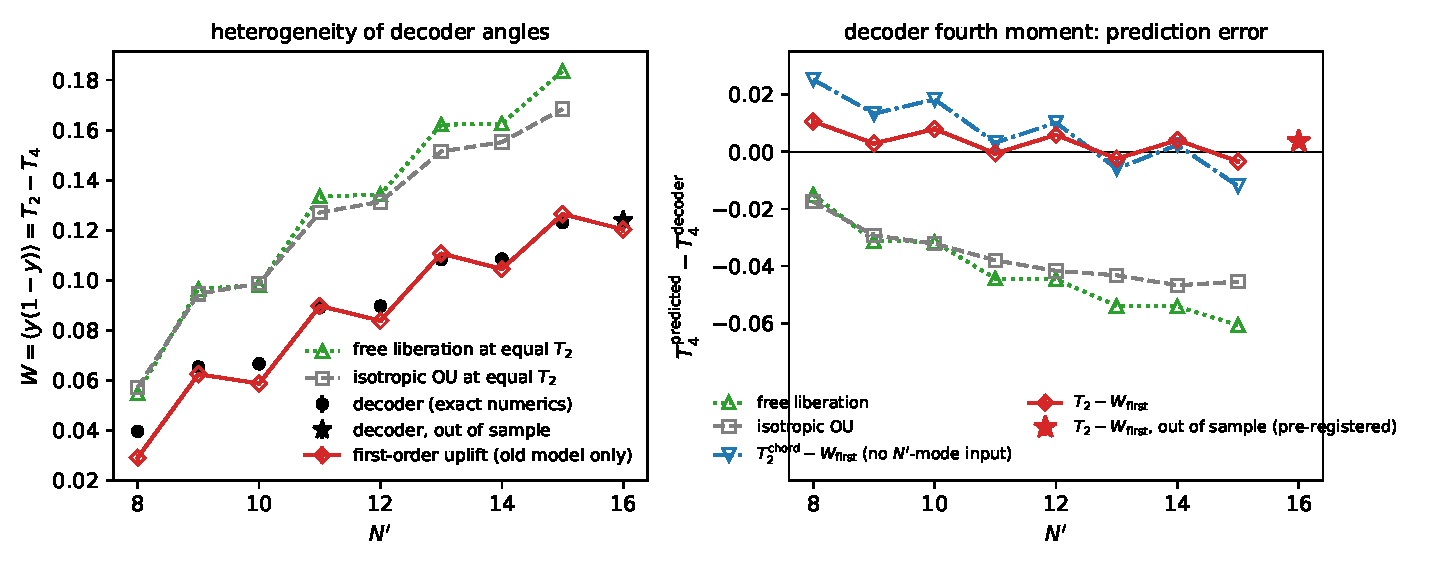
\includegraphics[width=\textwidth]{progress_2026-10-13_figs/fig_heterogeneity.pdf}
\caption{(a)~Heterogeneity $W=T_2-T_4$ of the decoder (black) and its first-order prediction $\Wone$ from the old model (red).
Free liberation and the isotropic OU curve at the decoder's $T_2$ are shown for comparison; the gap to the OU curve is
the localization. The star at $\Np=16$ is the exact decoder on the pre-registered realizations. (b)~Error of four
predictions of $T_4^\dec$: free liberation, isotropic OU, $T_2^\dec-\Wone$, and the parameter-free variant with $T_2$ from
the chord formula. The red star is the pre-registered out-of-sample test at $\Np=16$.}
\label{fig:heterogeneity}
\end{figure}

\paragraph{A parameter-free variant.} Eq.~\eqref{eq:prediction} still uses the measured $T_2^\dec$. For a prediction
with no input from the $\Np$-mode model, $T_2$ can be taken from the double-scaled chord formula of BLY~\cite{BLY}, which
the 29 September report found accurate to about 2\,\%. Writing $T_2=1-4b(1-b)(1-r)$ with $b=1-F/\Np$, $r$ is BLY's closed
form for the normalized two-point function at $\lambda_{\rm BLY}=2p^2/\Np$. The errors in $T_4$ become $+0.025$,
$+0.013$, $+0.018$, $+0.003$, $+0.010$, $-0.006$, $+0.002$, $-0.012$ for $\Np=8$--$15$, i.e.\ at most 2.7\,\% of $T_4$ for
$\Np\ge11$. They are dominated by the 1--2\,\% error of the chord $T_2$.

\subsection{An out-of-sample test at \texorpdfstring{$\Np=16$}{N'=16}}\label{sec:N16}

\PRE\ Before diagonalizing any $\Np=16$ decoder, we wrote down predictions in
\path{results/data/uplift_2026-10-12/prereg_N16.json}. They used only first-order data from the $N=15$ model (three
realizations) and the calibration of $\Np=10$--$15$. We then ran the exact $\Np=16$ decoder ($D=12870$, $d=4374$) for two
of those realizations, at a peak memory of 10.8\,GB each. Table~\ref{tab:prereg} lists the outcome. The main prediction, for
the residual of the heterogeneity and hence for $T_4$, passed in both realizations: $T_4$ was predicted to $+0.003$ and
$+0.004$. Two side predictions, for the precise wall fractions and for the fraction of states with $y<\tfrac12$, missed
narrowly. The exact decoder is slightly more enhanced at the walls than the calibration assumed.

\begin{table}[ht]
\centering\small
\caption{Pre-registered predictions at $\Np=16$ and their outcomes (realizations with seeds 9000 and 9001).}
\label{tab:prereg}
\begin{tabular}{@{}>{\raggedright\arraybackslash}p{0.44\textwidth}>{\raggedright\arraybackslash}p{0.27\textwidth}>{\raggedright\arraybackslash}p{0.22\textwidth}@{}}\toprule
Prediction & Outcome & Verdict\\\midrule
P1: $W^\dec-\Wone\in[0,+0.005]$ (so $T_4$ to $\le0.005$) & $+0.0030$, $+0.0042$ & pass\\
P2: no exact atoms & 0, 0 & pass\\
P3: wall fractions 5--20\,\% above first order & ratios 1.16--1.26 & narrow misses at thresholds $0.03$, $0.01$\\
P4: KS distance of $\min(y,1-y)\le0.035$; of $y\ge0.05$; fraction $y<\tfrac12$ in $[0.36,0.40]$ & 0.018, 0.025; 0.088, 0.107; 0.367, 0.358 & one narrow miss\\
P5: $T_2\in[0.585,0.615]$ & 0.6075, 0.6119 & pass\\\bottomrule
\end{tabular}
\end{table}

%=====================================================================
\section{Why the first-order heterogeneity works, and its limits}\label{sec:why}
%=====================================================================

\subsection{First order is wrong about \texorpdfstring{$T_2$}{T2} but right about \texorpdfstring{$W$}{W}}

The success of $\Wone$ is not an identity. First order underestimates $T_2$ itself by 5--11\,\%. The block form of
\S\ref{sec:decoder} lets us split the difference between first order and the exact decoder into two steps.
\emph{Self-dressing} keeps the diagonal blocks of the pencil~\eqref{eq:pencilG}--\eqref{eq:pencil} exact but drops the
off-diagonal block.
\emph{Mixing} restores the off-diagonal block. Table~\ref{tab:blocks} shows both steps.

\begin{table}[ht]
\centering\small
\caption{First order $\to$ self-dressed (diagonal blocks of~\eqref{eq:pencilG}--\eqref{eq:pencil}) $\to$ exact, averaged over two
realizations. ``Mixing'' is the term $2\|C\|_F^2/d$ of~\eqref{eq:T2mix}.}
\label{tab:blocks}
\begin{tabular}{lccccccc}\toprule
& \multicolumn{3}{c}{$T_2$} & & \multicolumn{3}{c}{$W$}\\\cmidrule{2-4}\cmidrule{6-8}
$\Np$ & first & self & exact & mixing & first & self & exact\\\midrule
10 & 0.699 & 0.734 & 0.748 & 0.014 & 0.0578 & 0.0624 & 0.0664\\
11 & 0.642 & 0.670 & 0.678 & 0.008 & 0.0885 & 0.0886 & 0.0871\\
12 & 0.621 & 0.662 & 0.678 & 0.016 & 0.0850 & 0.0854 & 0.0894\\
13 & 0.560 & 0.600 & 0.613 & 0.012 & 0.1118 & 0.1113 & 0.1092\\
14 & 0.573 & 0.624 & 0.640 & 0.016 & 0.1042 & 0.1033 & 0.1071\\
15 & 0.538 & 0.582 & 0.594 & 0.012 & 0.1269 & 0.1244 & 0.1229\\\bottomrule
\end{tabular}
\end{table}

Self-dressing raises $T_2$ substantially, by $0.03$--$0.05$, as Proposition~\ref{prop:monotone} requires. Yet it moves $W$
by at most $0.003$ for $\Np\ge11$. Mixing raises $T_2$ by another $0.008$--$0.016$, as~\eqref{eq:T2mix} requires. It
moves $W$ by about $+0.004$ at even $\Np$ and $-0.002$ at odd $\Np$, which is the parity-alternating residual of
Table~\ref{tab:prediction}.

The self-dressing step is captured by a simple mean-field rule. In~\eqref{eq:hfam2}, replace $R$ by its expectation
value $\rho_j=\ip{k_j}{Rk_j}/\|k_j\|^2$ in the first-order cloud $k_j=\Kh h_j$ of each singular vector. Then
\begin{equation}\label{eq:meanfield}
\mu_j=\frac{1-\sigma_j^2(1-\rho_j)/(1+\rho_j)^2}{1+\sigma_j^2/(1+\rho_j)}.
\end{equation}
This reproduces the self-dressed $T_2$ to within $0.005$ at $\Np=11$--$14$ \NUM. Physically, a fraction
$\rho_j/(1+\rho_j)$ of each cloud returns to the empty sector, and the total cloud shrinks by $1/(1+\rho_j)$.

\subsection{Per-state anatomy: a shift and a spread that cancel in \texorpdfstring{$W$}{W}}

To see why $W$ survives when $T_2$ does not, we tracked individual states. Each first-order state was projected onto the
exact BPS space, where it keeps 97\,\% of its norm on average, and then decomposed into exact decoder eigenvectors.
Figure~\ref{fig:mechanism} shows the result at $\Np=14$. A first-order state with value $y_1$ ends up, on average, at a
larger $y$: higher by about $0.11$ for $y_1<0.6$, with the shift falling to $0.006$ at the walls. It is also spread over a
band of width about $0.14$. The change of $y(1-y)$ therefore has opposite signs in different parts of the spectrum:
$+0.07$ for $y_1<0.1$, where the shift moves states into the intermediate region, and $-0.045$ around $y_1\approx0.65$,
where it moves them out. The two contributions cancel in the mean to $+0.003$. The first-order heterogeneity is accurate
because of this approximate cancellation, not because the first-order states are accurate.

\begin{figure}[t]
\centering
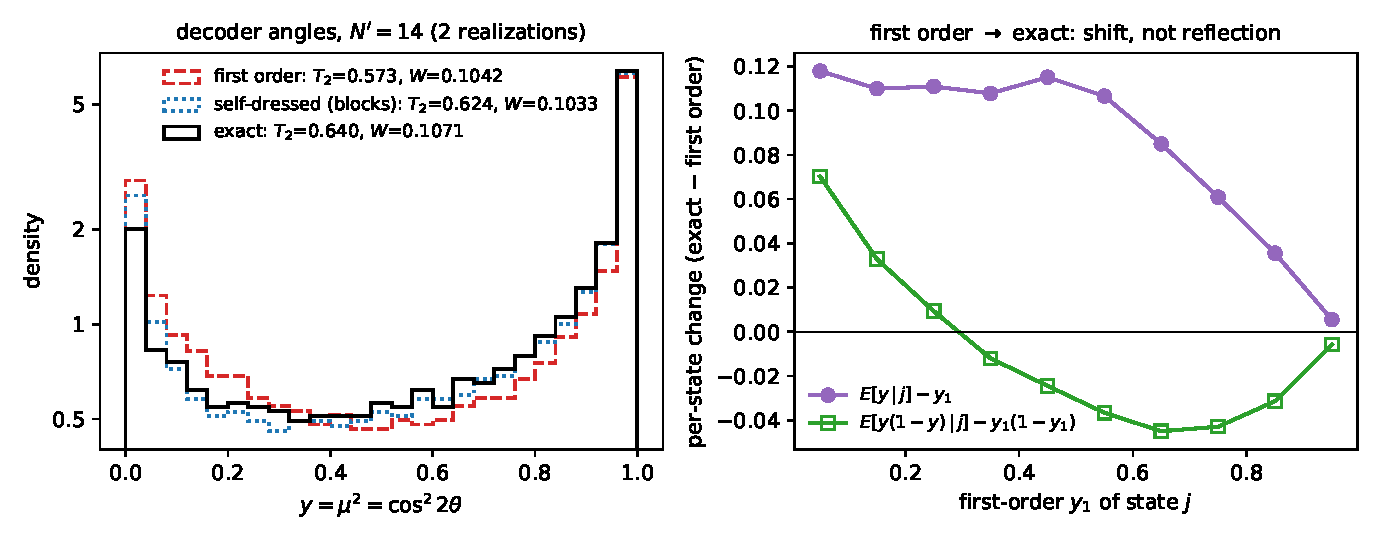
\includegraphics[width=\textwidth]{progress_2026-10-13_figs/fig_uplift_mechanism.pdf}
\caption{Anatomy of the first-order prediction at $\Np=14$ (two realizations, computed entirely from the old model via
the exact uplift). (a)~Distribution of $y$ at first order, after self-dressing, and exact. (b)~Per-state change from first
order to exact, binned in the first-order value $y_1$. $E[y|j]$ is the average of $y$ over the exact eigenvectors
weighted by their overlap with the first-order state $j$ (doubly stochastic weights). The shift in $y$ is positive
everywhere, while the change in $y(1-y)$ changes sign; their effects on $W$ cancel on average.}
\label{fig:mechanism}
\end{figure}

\subsection{The residual and its drift}

Measured on the same realizations, the residual $W^\dec-\Wone$ is nearly deterministic: its standard error over
realizations is $\le0.0013$. It has two components. Mixing alternates with parity, as above. Self-dressing contributes a slow drift: $+0.005$ at $\Np=10$, about
zero at $\Np=11$--$12$, and $-0.0025$ at $\Np=15$. The total residual on the same realizations is $+0.0093$, $+0.0079$, $+0.0045$,
$+0.0034$, $+0.0036$ at even $\Np=8$--$16$ and $+0.0020$, $-0.0012$, $-0.0026$, $-0.0039$ at odd $\Np=9$--$15$. So the odd-$\Np$
residual grows in magnitude. The agreement $W^\dec\approx\Wone$ is an empirical approximation at the sizes we can reach,
not an asymptotic statement. Whether it persists beyond $\Np=16$ is the most important caveat of this report. A
first-order computation at $\Np=17$ is feasible (about 11\,GB) and would give the next prediction in the odd sequence.
Testing it needs the exact $\Np=17$ decoder, which requires a more memory-efficient code.

\subsection{Two readings that did not survive}

\emph{Folding.} An earlier reading was that first order misplaces some states by the reflection $y\leftrightarrow1-y$,
which leaves $y(1-y)$ invariant. The folded distributions of $\min(y,1-y)$ do agree well, with Kolmogorov--Smirnov
distance $0.02$--$0.03$ for $\Np\ge13$ against $0.07$--$0.11$ for $y$. But the per-state tracking above shows a shift
and a spread, not a reflection, and we withdraw that reading.

\emph{Free rotation.} A natural null model is that $B$ is a \emph{free} rotation of the reference space
$\Hc_X\oplus\Hc_Y\wedge e$, on which the decoder is exactly $0$ or $1$. In exploratory scratch computations (not part of
the repository), both a scalar and an amalgamated free unitary Brownian rotation reproduced the self-liberation curve.
For example, at $\Np=10$ they gave $T_4=0.6515$ against $0.6519$ for liberation, at $T_2=0.75$. They missed the decoder by
the localization amount. The deformation of $B$ generated by the new couplings is therefore not free. Its non-free
content is the structure of \S\S\ref{sec:antiherm}--\ref{sec:decoder}.

%=====================================================================
\section{Discussion}\label{sec:discussion}
%=====================================================================

\subsection{What we have learned}

The decoder asks how much of a BPS state of the enlarged model is visible from the smaller model. Our answer is now
explicit. Every BPS state of the enlarged model is an old BPS state plus a dressing cloud, and the clouds are determined
by a linear system with an anti-Hermitian coupling. Using only the old model's metric, this resolves both ambiguities
that CV~\cite{CV} identified in the uplift of harmonic representatives (Corollary~\ref{cor:minnorm}). It also gives the decoder a closed form. To first order,
the principal angle of an uplifted state is the arctangent of its dressing amplitude, and the dressing cost is a
time-integrated two-point function of the new mode's pair operator.

Within this picture, the decoder's departure from an isotropic deformation has a precise meaning. The identity
$T_4=T_2-W$ turns it into a statement about the weight at intermediate angles. That weight is set by how the dressing
costs are distributed over old BPS states. The walls are a separate, arithmetic phenomenon, governed by a dimension count,
and they disappear at $\Np=15$ without taking localization with them. Quantitatively, the first-order dressing costs of
the smaller model predict the decoder's fourth moment an order of magnitude better than free liberation or isotropic
deformations. They also passed a pre-registered out-of-sample test.

\subsection{Towards a gravitational computation}

Proposition~\ref{prop:twopoint} turns the first-order decoder into a question of the kind the chord formalism answers.
What is the spectrum, on the BPS sector, of the time-integrated zero-temperature two-point function of a random
two-fermion matter operator? The first moment of that spectrum is an integrated two-point function. Its higher moments,
which fix $\Wone$, involve repeated insertions of $E$ separated by $H_0^{-1}$ and BPS projectors, so in chord language they
are matter-chord diagrams with energy denominators. The matter-chord machinery of BLY~\cite{BLY} and BINT~\cite{BINT}, extended by an
$H^{-1}$ insertion, is the natural tool. Carrying this out would make the prediction~\eqref{eq:prediction} fully
analytic. It would also connect localization to a bulk quantity, the distribution of the Euclidean ``time to dress'' a
BPS state. This identification is \INTERP; we have not attempted the chord calculation.

\subsection{A correction to the 5 October report}

The previous report stated that the localization term ``vanishes in strict double scaling.'' What was derived there is
an exact identity together with a leading-order argument for \emph{heavy} probes ($|A|\propto\sqrt N$ sites) in the
double-scaled limit with $p^2/N$ fixed. For the single-site decoder in that limit the decoder trivializes, so the statement
is empty there. Neither argument constrains the behavior at fixed $p=3$. The data now show no decrease of $L$ up to
$\Np=15$ ($0.043$, $0.047$, $0.045$ at $\Np=13$--$15$). The large-$N$ fate of localization at fixed $p$ is open.

\subsection{Open problems and next steps}

\begin{enumerate}\itemsep2pt
\item \textbf{Chord computation of the dressing-cost spectrum} (\S\ref{sec:twopoint}). This is the main analytic next step.
\item \textbf{Why $\Wone\approx W^\dec$.} The cancellation of \S\ref{sec:why} is observed, not derived. A first-order run
  at $\Np=17$ (old model $N=16$, about 11\,GB) would give the next odd-$\Np$ prediction. Testing it needs an exact
  $\Np=17$ decoder, and therefore a more memory-efficient code.
\item \textbf{The atom excess} over the refined bound (Table~\ref{tab:dims}). Some further algebraic constraint on
  $\Hc_X\cap\ker E$ is at work.
\item \textbf{Literature check} of the two-sided anti-Hermitian uplift and the orthogonal splitting, which have the flavor
  of a homological perturbation lemma.
\end{enumerate}

\appendix

%=====================================================================
\section{Verification summary}\label{app:verify}
%=====================================================================

\begin{table}[ht]
\centering\small
\caption{Numerical checks of the exact statements. Residuals are maxima over the sizes listed.}
\label{tab:verify}
\begin{tabular}{@{}>{\raggedright\arraybackslash}p{0.5\textwidth}>{\raggedright\arraybackslash}p{0.2\textwidth}l@{}}\toprule
Statement & Sizes & Residual\\\midrule
Uplift~\eqref{eq:uplift} spans the exact BPS space (full rank) & $\Np=8$--$10$, $12$--$14$ & $4.4\times10^{-15}$\\
Adjoint relation~\eqref{eq:adjoint} & $\Np=10$--$13$ & $6.4\times10^{-15}$ (relative)\\
Orthogonal splitting (Theorem~\ref{thm:split}) & $\Np=9$--$15$ & $1.1\times10^{-15}$\\
Closed-form pencil~\eqref{eq:pencilG}--\eqref{eq:pencil} $=$ exact decoder & $\Np=9$--$11$ (spectra); $10$--$15$ ($T_2$, 4 digits) & $10^{-10}$\\
Closed-form $h$-block vs.\ orthonormalized family & $\Np=10$--$13$ & $9.4\times10^{-15}$\\
Monotone self-dressing (Proposition~\ref{prop:monotone}) & $\Np=10$--$13$ & holds\\
Dressing cost $=$ spectrum of $P E^\dagger H_0^{-1}EP$ & $\Np=12$ & $10^{-9}$\\
Push-through form of the $h$-block & $\Np=12$ & $3\times10^{-15}$\\
Exact atoms $=$ first-order atoms ($\ker E$) & $\Np=8$--$16$ & identical counts\\
Even-$\Np$ block symmetry $\mathrm{spec}\,M_g=-\mathrm{spec}\,M_h$ & $\Np=10,12,14$ & $7.4\times10^{-15}$\\\bottomrule
\end{tabular}
\end{table}

%=====================================================================
\section{Numerical methods and reproducibility}\label{app:repro}
%=====================================================================

All intensive runs used the memory watchdog \path{scripts/memwatch.py}; the largest peak was 10.8\,GB (exact
$\Np=16$, cap 13\,GB). Couplings are standard complex Gaussians (\texttt{random\_couplings}, as in all project data),
the added mode is the last one, $p=3$ and $F=\lfloor\Np/2\rfloor$. The uplift computations use seeds $9000+r$. The OU
campaign at $\Np=15$ uses the seeds of~\cite{prog1005} with $s_0=0$ and $100$, and $K=8$ lags.

\begin{center}\small
\begin{tabular}{@{}>{\raggedright\arraybackslash}p{0.3\textwidth}>{\raggedright\arraybackslash}p{0.65\textwidth}@{}}\toprule
Item & Code and data\\\midrule
Exact uplift, closed form, first order & \path{src/uplift.py}; tests \path{tests/test_uplift.py}\\
Walls, first order and exact decoder (Tables~\ref{tab:dims},~\ref{tab:prediction}) & \path{scripts/run_uplift_walls.py}; data \path{results/data/uplift_2026-10-12/walls_N*.jsonl}\\
Block decomposition (Table~\ref{tab:blocks}) & \path{scripts/run_uplift_blocks.py}; \path{blocks.jsonl}\\
Prediction table and Fig.~\ref{fig:heterogeneity} & \path{scripts/analyze_uplift_heterogeneity.py}; \path{heterogeneity_analysis.json}\\
Figs.~\ref{fig:walls},~\ref{fig:densities},~\ref{fig:mechanism} & \path{scripts/plot_uplift_walls.py}, \path{plot_angle_densities.py}, \path{plot_uplift_mechanism.py}\\
$\Np=15$ OU campaign & \path{scripts/run_ou_fourarc.py}; \path{results/data/ou_fourarc_2026-10-05/N15_{a,b}/}, merged \path{ou_p3_N15_F7.jsonl}\\
Pre-registration ($\Np=16$) & \path{results/data/uplift_2026-10-12/prereg_N16.json} and its inputs\\
Derivations; research note & \path{docs/derivations.md} D6; \path{research/notes/uplift_localization_2026-10-12.md}\\\bottomrule
\end{tabular}
\end{center}

\begin{thebibliography}{99}\small
\bibitem{CV} J.~Chryssanthacopoulos and D.~Vegh, \emph{Fortuity and fragility in supersymmetric SYK}, arXiv:2608.12160 (2026).
\bibitem{prog0929} \texttt{syk\_gravity} project, \emph{Progress report, 29 September 2026}, \path{research/pdfs/progress_2026-09-29.pdf}.
\bibitem{prog1005} \texttt{syk\_gravity} project, \emph{Progress report, 5 October 2026: chord number is chaos degree, and the decoder's fourth moment is free liberation plus localization}, \path{research/pdfs/progress_2026-10-05.pdf}.
\bibitem{BBNR} M.~Berkooz, N.~Brukner, V.~Narovlansky and A.~Raz, \emph{The double scaled limit of super-symmetric SYK models}, JHEP 12 (2020) 110, arXiv:2003.04405.
\bibitem{BLY} J.~Boruch, H.~W.~Lin and C.~Yan, \emph{Exploring supersymmetric wormholes in $\mathcal N=2$ SYK with chords}, JHEP 12 (2023) 151, arXiv:2308.16283.
\bibitem{LMRS} H.~W.~Lin, J.~Maldacena, L.~Rozenberg and J.~Shan, \emph{Looking at supersymmetric black holes for a very long time}, SciPost Phys.\ \textbf{14} (2023) 128, arXiv:2207.00408.
\bibitem{FGMS} W.~Fu, D.~Gaiotto, J.~Maldacena and S.~Sachdev, \emph{Supersymmetric Sachdev-Ye-Kitaev models}, Phys.\ Rev.\ D \textbf{95} (2017) 026009, arXiv:1610.08917.
\bibitem{BINT} M.~Berkooz, M.~Isachenkov, V.~Narovlansky and G.~Torrents, \emph{Towards a full solution of the large $N$ double-scaled SYK model}, JHEP 03 (2019) 079, arXiv:1811.02584.
\bibitem{DHH} N.~Demni, T.~Hamdi and T.~Hmidi, \emph{On the spectral distribution of the free Jacobi process}, arXiv:1204.6227.
\end{thebibliography}

\end{document}
